\fenicschapter{Unicorn: A Unified Continuum Mechanics Solver}
              {Unicorn: A Unified Continuum Mechanics Solver}
              {Johan Hoffman, Johan Jansson, Niclas Jansson and Murtazo Nazarov}
              {hoffman-2}

\section{Introduction}

Unicorn is solver technology (models, methods, algorithms and software
implementations) with the goal of automated simulation of realistic
continuum mechanics applications, such as drag/lift computation for
fixed or flexible objects (fluid-structure interaction) in turbulent
incompressible or compressible flow (airplane/bird flight, car
aerodynamics). The basis for Unicorn is Unified Continuum (UC)
modeling formulated in Euler (laboratory) coordinates, together with a
G2 (General Galerkin) adaptive stabilized FEM discretization with a
moving mesh for tracking the phase interfaces. The UC model consists
of canonical conservation equations for mass, momentum, energy and
phase over the whole domain as one continuum, together with a Cauchy
stress and phase variable as data for defining material properties and
constitutive equation. Unicorn formulates and implements the adaptive
G2 method applied to the UC model, and interfaces to other components
in the FEniCS chain (FIAT, FFC, DOLFIN) providing representation of
finite element function spaces, weak forms and mesh, and algorithms
such as automated parallel assembly and linear algebra.

Unicorn as part of the FEniCS framework realizes automated
computational modeling for general continuum mechanics applications in
the form of canonical UC formulation in Euler coordinates,
duality-based adaptive error control, tensor assembly, time-stepping,
adaptive fixed-point iteration for solving discrete systems, mesh
adaptivity by local cell operations (split, collapse, swap) (through
MAdLib) and cell quality optimization (smoothing).

This chapter provides a description of the technology in Unicorn
focusing on simple, efficient and general algorithms and software
implementation of the UC concept and the adaptive G2
discretization. We describe how Unicorn fits into the FEniCS
framework, how it interfaces to other FEniCS components and what
interfaces and functionality Unicorn provides itself and how the
implementation is designed. We also give use case application examples
in fluid-structure interaction and adaptivity.

For a more detailed discussion on turbulence and adaptive error
control in continuum mechanics we refer to
chapter \ref{chapter:applications:fsi}.

\begin{figure}[!h]
\center{
\boxed{
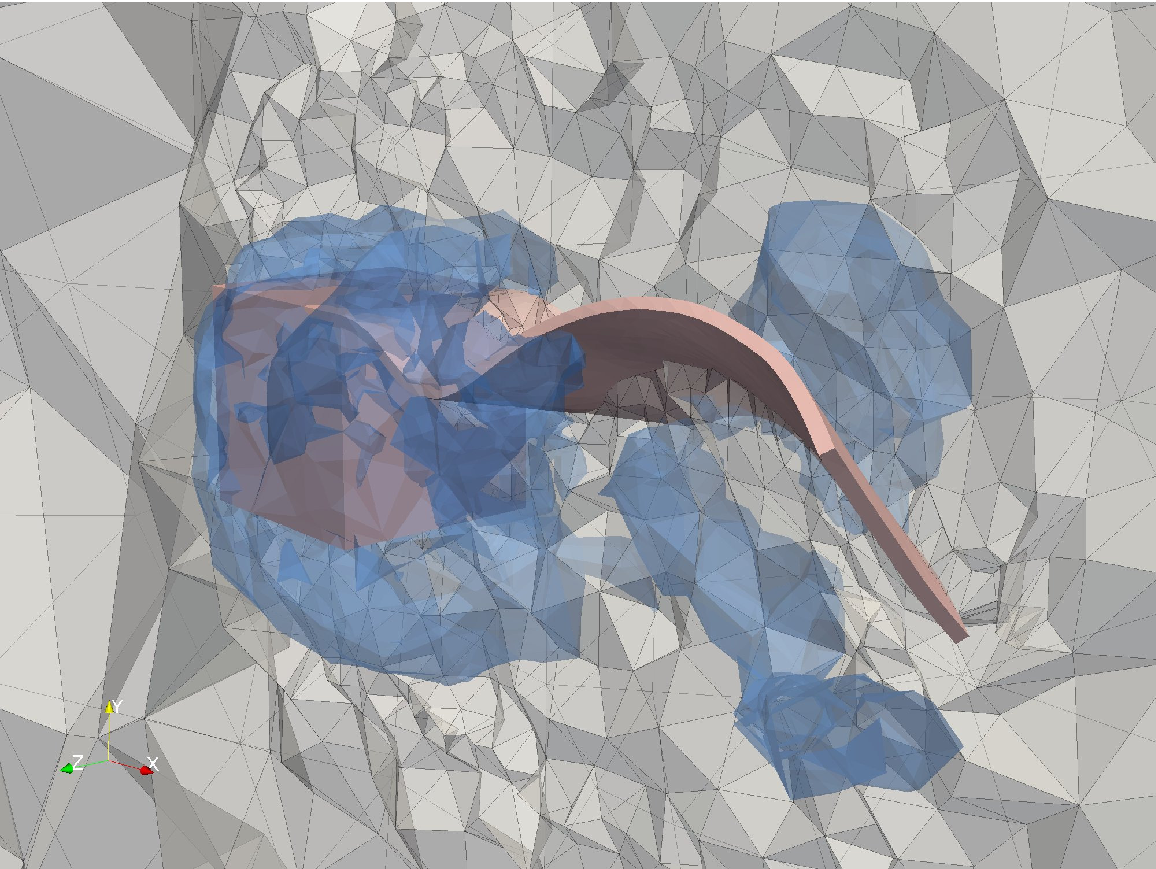
\includegraphics[width=12cm]{chapters/hoffman-2/pdf/cube556.pdf}
}}
%\includegraphics[width=10cm]{media/unicorn_fsi_flag3D_01.pdf}
\caption{
A fluid-structure example application of a flag mounted behind a cube in turbulent flow. The fluid-structure interface, an isosurface of the pressure and a cut of the mesh is plotted.
}
\label{fig:flag3D}
\end{figure}

The Unicorn software is organized into three parts:
\begin{description}
\item[Library]
The Unicorn library publishes interfaces to and implements common
solver technology such as automated time-stepping, error
estimation/adaptivity, mesh smoothing/adaptation interface and
slip/friction boundary condition.
\item[Solver]
The Unicorn solver implements the G2 adaptive discretization method
for the UC model by formulating the relevant weak forms and using the
solver technology in the library and from other components of
FEniCS. Currently there are two primary solvers: incompressible
fluid/solid (including fluids-structure interaction) and compressible
Euler (only fluid), where the long term goal is a unification of the
incompressible/compressible formulations as well.
\item[Applications]
Associated to the solver(s) are applications such as computational
experiments/benchmarks with certain geometries, coefficients and
parameters. These are represented as stand-alone programs built on top
of the Unicorn solver/library, running in either serial or parallel
(restricted to adaptive incompressible flow currently).
\end{description}

\begin{figure}[!h]
\center{
\boxed{
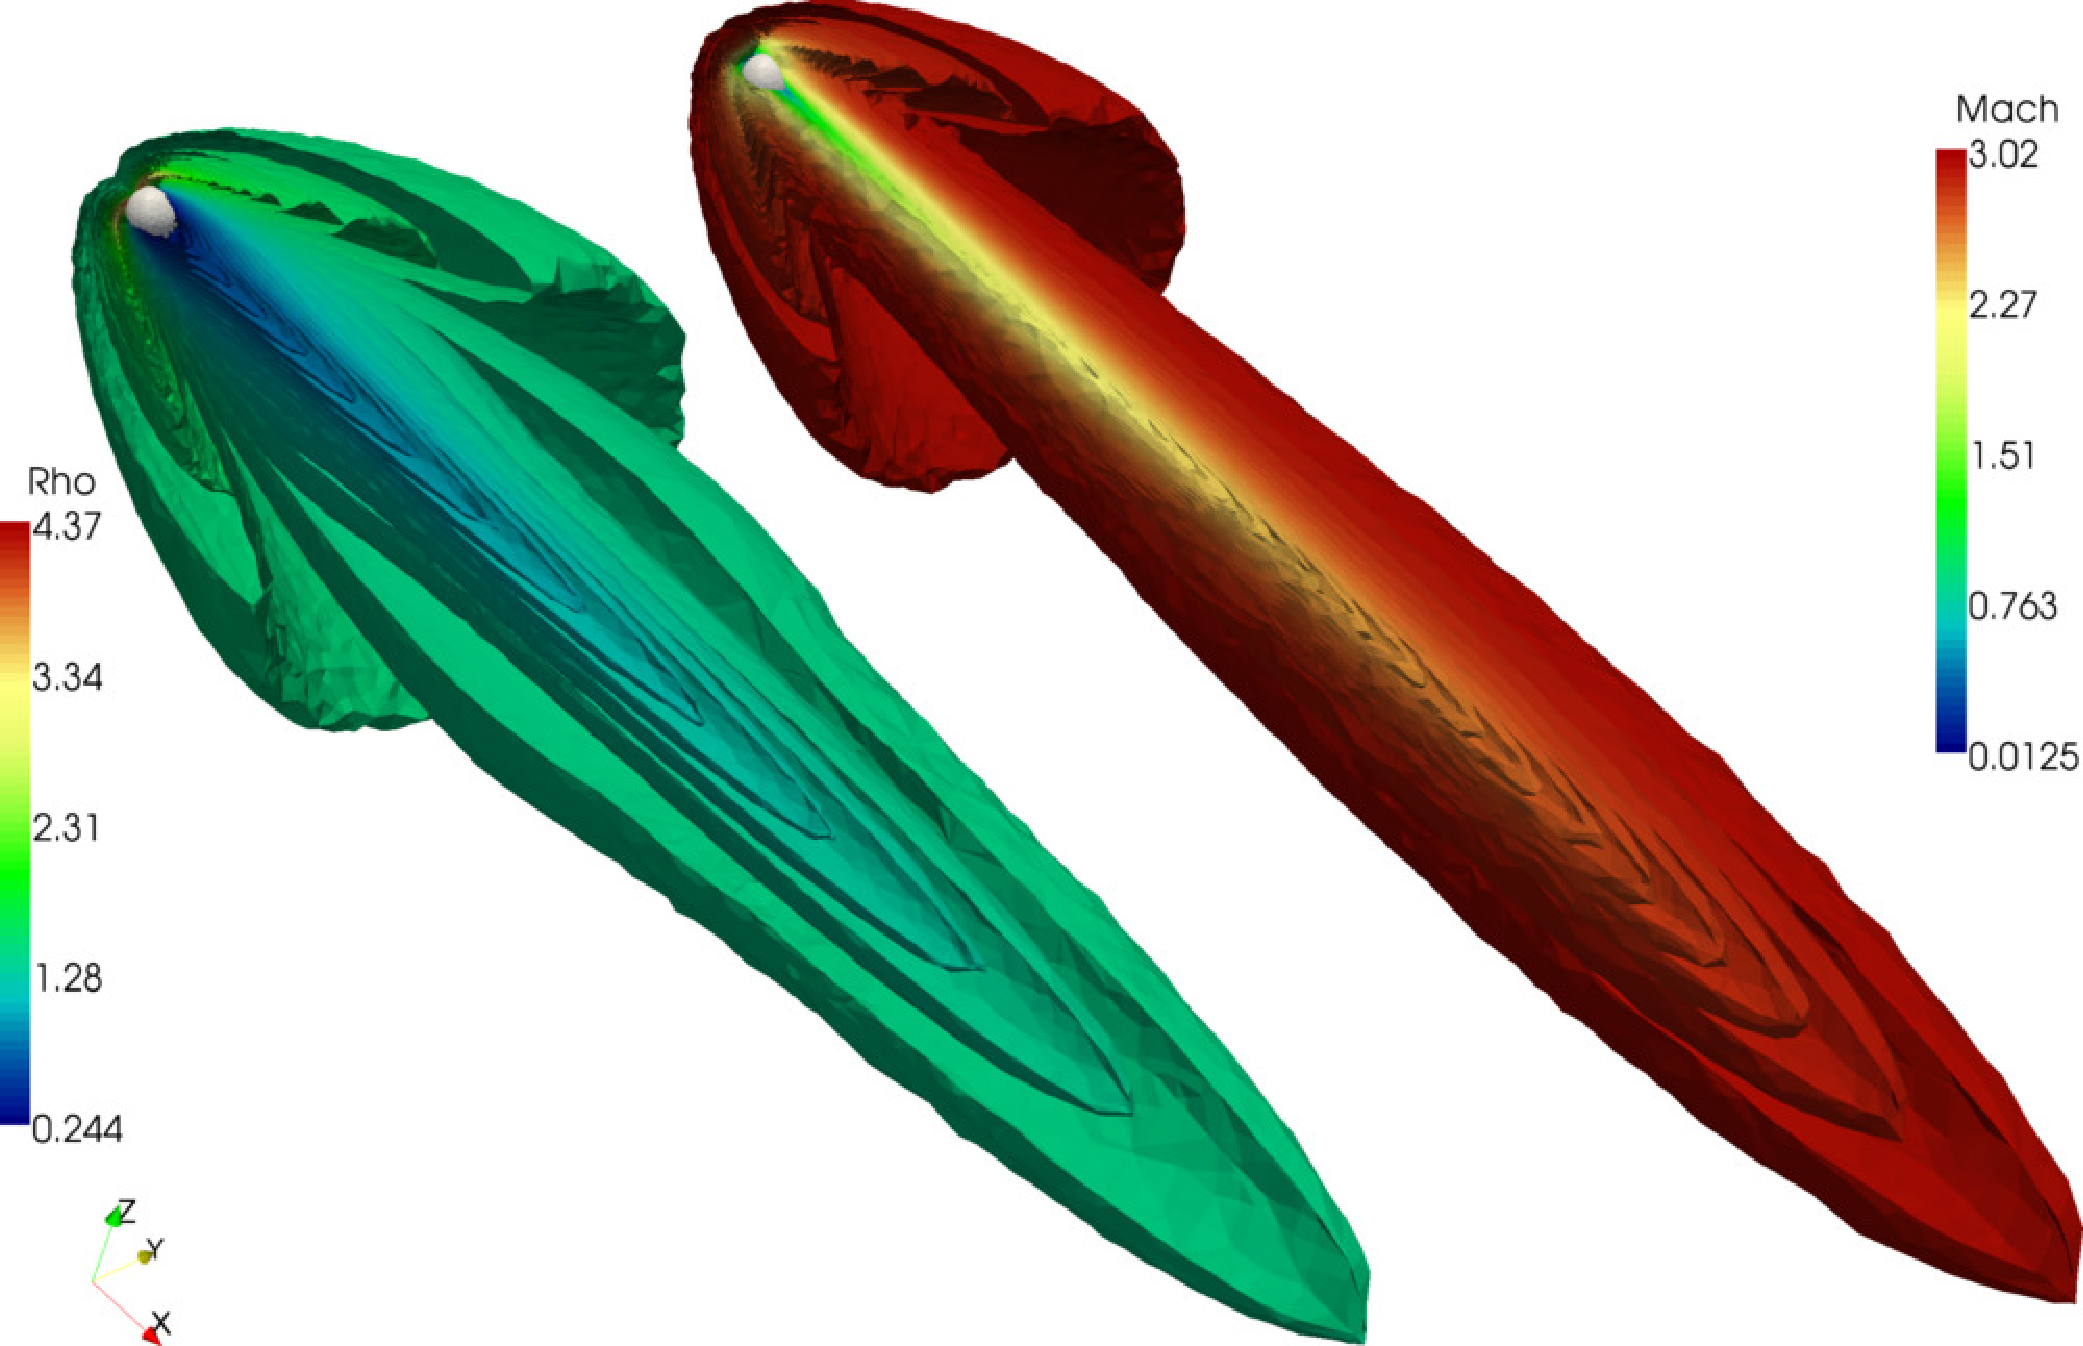
\includegraphics[width=12cm]{chapters/hoffman-2/pdf/compressible3D.pdf}
}}
%\includegraphics[width=10cm]{media/unicorn_fsi_flag3D_01.pdf}
\caption{
Example application of adaptive computation of 3D compressible flow
around a sphere.  }
\label{fig:compr3D}
\end{figure}

\begin{figure}[!h]
\center{
\boxed{
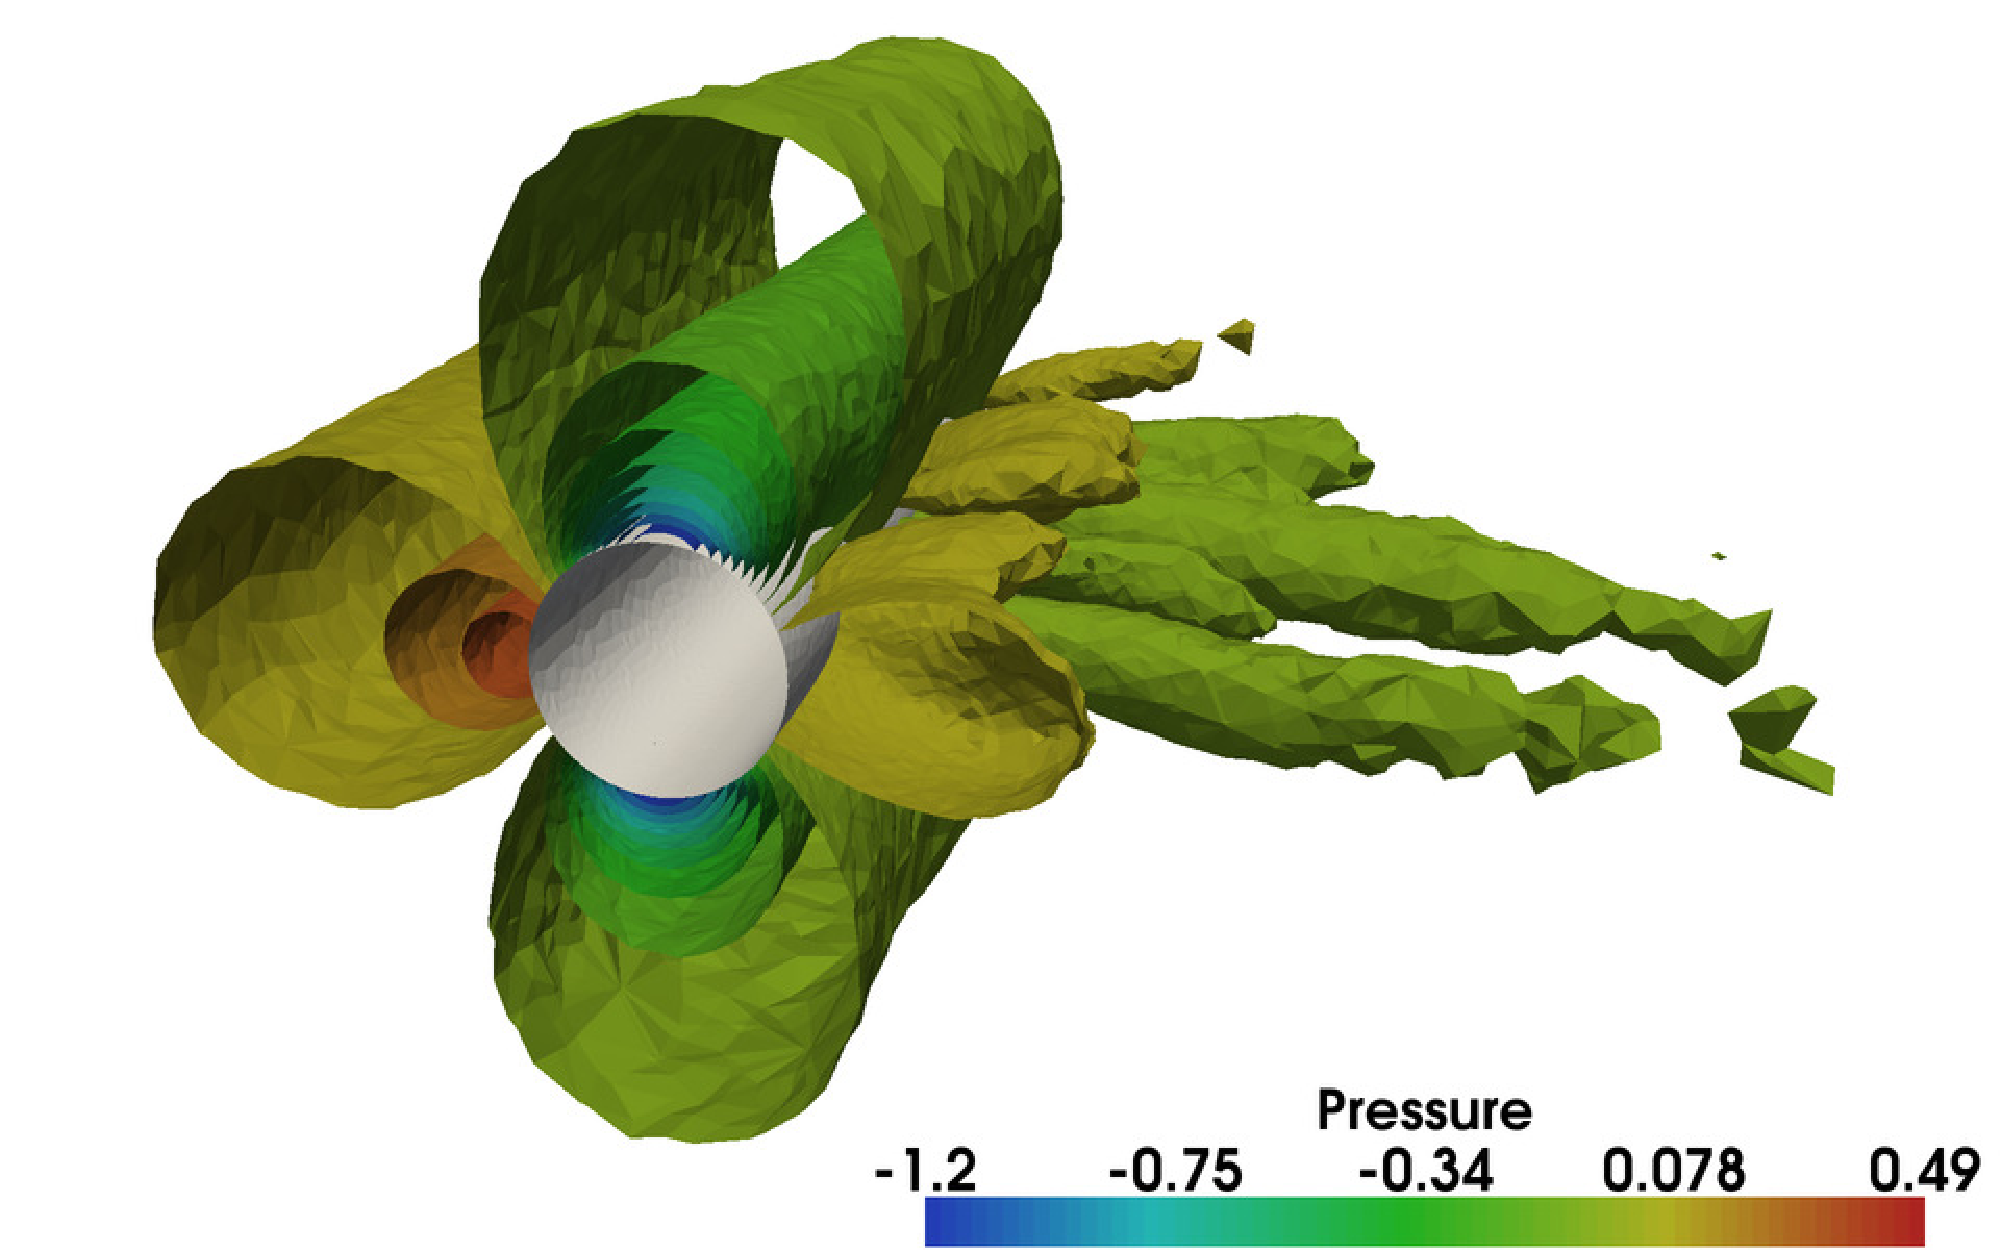
\includegraphics[width=12cm]{chapters/hoffman-2/pdf/Hoffman_fig3d.pdf}
}}
%\includegraphics[width=10cm]{media/unicorn_fsi_flag3D_01.pdf}
\caption{
Example application of 3D turbulent incompressible flow around a
cylinder with parallel adaptive computation. }
\label{fig:parcyl3D}
\end{figure}


\label{chapter:implementation:unicorn}


%[Implementation: TimeDependentPDE, error estimation based on duality,
%mesh adaptivity/smoothing, friction BC, solver interface, efficient
%solution of discrete systems by fixed-point iteration, parallel
%solver/mesh refinement.]

%Write a short introduction to your chapter here. Explain the purpose
%of the chapter and include a brief outline. Remember to index
%important terms and use citations.~\cite{Ciarlet1978}

%\index{important term}

\section{Acknowledgement}

We acknowledge contributions to Unicorn, both software development as
well as ideas and scientific support from: Mattias Aechtner, Peter
Brune, Zilan Ciftci, G\"aetan Compere, Niyazi Cem Degirmenci, Vida
Heidarpour Dehkordi, Claes Johnson, Ashraful Kadir, Mohammad Reza
Mokhtari, Jeannette Sp\"uhler, Michael St\"ockli and Rodrigo Vilela de
Abreu.

\section{Notation}

We occasionally use an indexed Einstein notation with the derivative of a
function $f$ with regard to the variable $x$ denoted as $D_x f$, and
the derivative with regard to component $x_i$ of component $f_j$
denoted as $D_{x_i} f_j = \nabla f_j$. Repeated indices denote a sum:
$D_{x_i} f_i = \sum_{i=1}^d D_{x_i} f_i = \nabla \cdot f$. Similarly
we can express derivatives with respect to any variable: $D_u u = 1$.
%------------------------------------------------------------------------------
\section{Unified Continuum modeling}

% Intro (explain mesh motion)

We define a unified continuum model in a fixed Euler
coordinate system consisting of:
\begin{itemize}
\item
conservation of mass
\item
conservation of momentum
\item
conservation of energy
\item
phase convection equation
\item
constitutive equations for stress as data
\end{itemize}
where the stress is the Cauchy (laboratory) stress and the phase
variable is used to define material data such as constitutive equation
for the stress and material parameters. Note that in this continuum
description the coordinate system is fixed (Euler), and a phase
function (marker) is convected according to the phase convection
equation.

We define two variants of this model: incompressible and compressible,
where a future aim is to construct a unified
incompressible/compressible model and solver.

We start with a model for conservation of mass, momentum and energy,
together with a convection equation for a phase function $\theta$ over
a space-time domain $Q = \Omega \times [0, T]$ with $\Omega$ an open
domain in $R^3$ with boundary $\Gamma$:
\begin{equation}
  \addtolength{\fboxsep}{5pt}
  \boxed{
    \begin{split}\label{eq:TotalModel}
      D_t \rho + D_{x_j} (u_j \rho) &= 0
      \quad \text{(Mass conservation)}\\
      D_t m_i + D_{x_j} (u_j m_i) &= D_{x_j} \sigma_i
      \quad \text{(Momentum conservation)}\\
      D_t e + D_{x_j} (u_j e) &= D_{x_j} \sigma_i u_i
      \quad \text{(Energy conservation)}\\
      D_t \theta + D_{x_j} u_j \theta &= 0
      \quad \text{(Phase convection equation)}
    \end{split}
  }
\end{equation}
together with initial and boundary conditions. We can then pose
constitutive relations between the constitutive (Cauchy) stress
component $\sigma$ and other variables such as the velocity $u$.

We define incompressibility as:
\begin{align*}
D_t \rho + u_j D_{x_j} \rho &= 0
\end{align*}

which together with mass and momentum conservation gives:
\begin{align*}
\rho(D_t u_i + u_j D_j u_i) &= D_{x_j} \sigma_{ij}\\
D_{x_j} u_j &= 0
\end{align*}
where now the energy equation is decoupled and we can omit it.

We decompose the total stress into constitutive and forcing stresses:
\begin{align*}
D_{x_j} \sigma_{ij} = D_{x_j} \sigma_{ij} + D_{x_j} \sigma^f_{ij} =
D_{x_j} \sigma_{ij} + f_i
\end{align*}

Summarizing, we end up with the incompressible UC formulation:
\begin{equation}
  \addtolength{\fboxsep}{5pt}
  \boxed{
    \begin{split}\label{eq:TotalUC}
      \rho(D_t u_i + u_j D_{x_j} u_i) &= D_{x_j} \sigma_{ij} + f_i\\
      D_{x_j} u_j &= 0\\
      D_t \theta + D_{x_j} u_j \theta &= 0
    \end{split}
  }
\end{equation}
The UC modeling framework is simple and compact, close to the
formulation of the original conservation equations, without mappings
between coordinate systems. This allows simple manipulation and
processing for error estimation and implementation. It is also
general, we can choose the constitutive equations to model simple or
complex solids and fluids, possibly both in interaction, with
individual parameters.

\subsection{Automated computational modeling and software design}

One key design choice of UC modeling is to define the Cauchy stress
$\sigma$ as data, which means the conservation equations are fixed
regardless of the choice of constitutive equation. This gives a
generality in method and software design, where a modification of
constitutive equation impacts the formulation/implementation of the
constitutive equation, but not the formulation/implementation of the
conservation equations.

In Unicorn we choose an Euler coordinate system and moving mesh,
allowing a unified/canonical formulation of conservation
equations. This enables automated computational modeling (with
discretization and error control) for full fluid-structure (or
multi-phase) problems, rather than to one component at a time, with
unclear strategy how to combine them. We believe this is a unique
method/software system in this respect.

\section{Space-time General Galerkin discretization}

The General Galerkin (G2) method has been developed as an adaptive
stabilized finite element method for turbulent
incompressible/compressible flow
\cite{Hoffman2005,HoffmanJohnson2006b,Hoffman2006,Hoffman2009,Hoffman2006b,Nazarov2009}
G2 has been shown to be cheap, since the adaptive mesh refinement is
minimizing the number of degrees of freedom, general, since there are
no model parameters to fit, and reliable, since the method is based on
quantitative error control in a chosen output. The G2 method has been
shown to accurately compute quantities of interest in both laminar and
turbulent
flow \cite{Hoffman2005,HoffmanJohnson2006b,Hoffman2006,Hoffman2009,Hoffman2006b,HoffmanJanssonEtAl2009}.

We begin by describing the standard FEM applied to the model to
establish basic notation, and proceed to describe streamline diffusion
stabilization and local ALE map over a mesh $T^h$ with mesh size h
together with adaptive error control based on duality.

\subsection{Standard Galerkin}

We begin by formulating the standard cG(1)cG(1) FEM
\cite{ErikssonEstepHansboEtAl1996} with piecewise continuous linear solution in time
and space for \ref{eq:TotalModel} by defining the exact solution: $w =
[u, p, \theta]$, the discrete solution $W = [U, P, \Theta]$, the
test function $v = [v^u, v^p, v^\theta]$ and the residual $R(W) =
[R_u(W), R_p(W), R_\theta(W)]$:

\begin{align*}
  R_u(W) &= \rho(D_t U_i + U_j D_{x_j} U_i) - D_{x_j} \Sigma_{ij} - f_i\\
  R_p(W) &= D_{x_j} U_j\\
  R_\theta(W) &= D_t \Theta + u_j D_{x_j} \Theta
\end{align*}

where $R(w) = 0$ and $\Sigma$ denotes a discrete piecewise constant
stress.

To determine the degrees of freedom $\xi$ we enforce the Galerkin
orthogonality $(R(W), v) = 0, \forall v \in V_h$ where $v$ are test
functions in the space of piecewise linear continuous functions in
space and piecewise constant discontinuous functions in time and
$(\cdot,\cdot)$ denotes the space-time $L_2$ inner product over Q. We
thus have the weak formulation:

\begin{align*}
  (R^u(W), v^u) &= (\rho(D_t U_i + U_j D_j U_i) - f_i, v^u_i) + (\Sigma_{ij}, D_{x_j} v^u_i) - \int_{t_{n-1}}^{t_n}\int_\Gamma \Sigma_{ij} v^u_i n_j ds dt = 0\\
  (R^p(W), v^p) &= (D_{x_j} U_j, v^p) = 0\\
  (R^\theta(W), v^\theta) &= (D_t \Theta + u_j D_{x_j} \Theta, v^\theta) = 0
\end{align*}

for all $v \in V_h$, where the boundary term on $\Gamma$ arising from
integration by parts vanishes if we assume a homogenous Neumann
boundary condition for the stress $\Sigma$.

This standard finite element formulation is unstable for
convection-dominated problems and due to choosing equal order for the
pressure and velocity. Thus we cannot use the standard finite element
formulation by itself but proceed to a streamline diffusion
stabilization formulation. We also describe a local ALE discretization
for handling the phase interface.

\subsection{Local ALE}

If the phase function $\Theta$ has different values on the same cell
it would lead to an undesirable diffusion of the phase interface. By
introducing a local ALE coordinate map \cite{ErikssonEstepHansboEtAl1996} on
each discrete space-time slab based on a given mesh velocity (i.e. the
material velocity of one of the phases) we can define the phase
interface at cell facets, allowing the interface to stay
discontinuous. We describe the details of the coordinate map and its
influence on the FEM discretization
in \cite{HoffmanJanssonLoggEtAl2009}. The resulting discrete phase
equation is:
\begin{equation}
\begin{split}\label{eq:ALE}
D_t \Theta(x) +
(U(x) - \beta_h(x)) \cdot \nabla \Theta(x) = 0
\end{split}
\end{equation}
with $\beta_h(x)$ the mesh velocity.

We thus choose the mesh velocity $\beta_h$ to be the discrete material
velocity U in the structure part of the mesh (vertices touching
structure cells) and in the rest of the mesh we use mesh smoothing to
determine $\beta_h$ to maximize the mesh quality according to a chosen
objective, alternatively use local mesh modification operations
(refinement, coarsening, swapping) on the mesh to maintain the quality
\cite{Comp`ereRemacleJanssonEtAl2009}. Note that we still compute in Euler
coordinates, but with a moving mesh.

\subsection{Streamline diffusion stabilization}

For the standard FEM formulation of the model we only have stability
of $U$ but not of spatial derivatives of $U$. This means the solution
can be oscillatory, causing inefficiency by introducing unnecessary
error. We instead choose a weighted standard Galerkin/streamline
diffusion method of the form $(R(W), v + \delta R(v)) = 0, \forall v
\in V_h$ (see \cite{ErikssonEstepHansboEtAl1996}) with $\delta > 0$ a stabilization
parameter. We here also make a simplification where we only introduce
necessary stabilization terms and drop terms not contributing to
stabilization. Although not fully consistent, the streamline diffusion
stabilization avoid unnecessary smearing of shear layers as the
stabilization is not based on large ($\approx h^{-\frac{1}{2}}$) cross flow
derivatives). For the UC model the stabilized method thus looks like:

\begin{align*}
  (R^u(W), v^u) &= (\rho(D_t U_i + U_j D_j U_i) - f_i, v^u_i) + (\Sigma_{ij}, D_{x_j} v^u_i) + SD^u(W, v^u) = 0\\
  (R^p(W), v^p) &= (D_{x_j} U_j, v^p) + SD^p(W, v^p) = 0
\end{align*}
for all $v \in V_h$, and:
\begin{align*}
  SD^u(W, v^u) &= \delta_1 (U_j D_j U_i, U^u_j D_j v^u_i) +
  \delta_2 (D_{x_j} U_j, D_{x_j} v^u_j)\\
  SD^p(W, v^p) &= \delta_1 (D_{x_i} P, D_{x_i} v^p)
\end{align*}

where we only include the dominating stabilization terms to reduce
complexity in the formulation.

\subsection{Duality-based adaptive error control}

We give a summary for illustrative purposes of the mathematical
framework for duality based error estimation in the context of the UC
formulation.

We consider an equation (such as the UC) in residual form $R(u) =
0$. We define a linearized operator satisfying: $A(\bar{U})e =
R(U)$. We can then construct an error estimate as follows, where
$\psi$ is the quantity of interest.

It is of critical importance in science and engineering to be able to
bound the computational error $e = u - U$, we can phrase this as
requiring that $e$ satisfies:
\begin{align}
|(e, \psi)| &< TOL
\end{align}
We define:
\begin{displaymath}
  \begin{split}
    (Aw, v) &= (w, A^* v) \quad \text{(adjoint definition)}\\
    A^* \phi &= \psi \quad \text{(dual equation)}
  \end{split}
\end{displaymath}
We can then express the error in terms of the residual and dual solution:
\begin{displaymath}
  \begin{split}
    (e, \psi) &= (e, A^*\phi) = (Ae, \phi) = (-R(U), \phi)  \quad \text{(error representation)}\\
  \end{split}
\end{displaymath}
We note we could alternatively start from the weak formulation:
\begin{displaymath}
  \begin{split}
(e, \psi) = a^*(\phi, e) = a(e, \phi) = (-R(U), \phi)\\
  \end{split}
\end{displaymath}
% Space-time interpolation with h ``space-time'' mesh size?
We thus have a canonical formula for the error estimate:
\begin{displaymath}
  \begin{split} |(e, \psi)| &\leq \sum_K \|h R(U)\|_K \|D \phi\|_K
  = \sum_K {\cal E}_K \quad \text{(error bound)} \end{split}
\end{displaymath}
where ${\cal E}_K$ is an error indicator on each cell $K$.

We can thus define an adaptive algorithm for controlling
$|(e, \psi)|$ by making sure that $U$ satisfies:
\begin{align*}
\sum_K {\cal E}_K &< TOL\\
&\Rightarrow\\
|(e, \psi)| &< TOL
\end{align*}

by iteratively reducing $h$ in cells with large ${\cal E}_K$ until the
tolerance condition is satisfied.

\subsection{Unicorn/FEniCS software implementation}

We implement the G2 discretization of the UC (including adaptive error
control) in a general interface for time-dependent PDE where we give
the forms $a(U, v) = (D_U F_U, v)$ and $L(v) = (F_U, v)$ for
assembling the linear system given by Newton's method for a time step
for the incompressible UC with Newtonian fluid constitutive equation
in figure \ref{code:FFC_UC}. The language used is the FEniCS Form
Compiler (FFC) \cite{KirbyLogg2006} form notation. In the adaptive error
control, we similarly represent residuals as forms in the form
language, which then allows us to compute error indicators using basic
programming constructs.

An overview of the interfaces and implementations of the Unicorn data
structures and algorithms are presented below.

\begin{figure}[!h]
\center{
\lstset{language=Python,frame=ltrb,framesep=5pt,basicstyle=\footnotesize,
 keywordstyle=\ttfamily\color{OliveGreen},
 identifierstyle=\ttfamily\color{CadetBlue}\bfseries,
 commentstyle=\color{Brown},
 stringstyle=\ttfamily,
 showstringspaces=ture}

\begin{lstlisting}

...

def ugradu(u, v):
    return [dot(u, grad(v[i])) for i in range(d)]

def epsilon(u):
    return 0.5 * (grad(u) + transp(grad(u)))

def S(u, P):
    return mult(P, Identity(d)) - mult(nu, grad(u))

def f(u, v):
    return -dot(ugradu(Uc, Uc), v) + \
        dot(S(Uc, P), grad(v)) + \
	-mult(d1, dot(ugradu(Um, u), ugradu(Um, v))) + \
	-mult(d2, dot(div(u), div(v))) + \
        dot(ff, v)

def dfdu(u, k, v):
    return -dot(ugradu(Um, u), v) + \
        -dot(mult(nu, grad(u)), grad(v)) + \
        -mult(d1, dot(ugradu(Um, u), ugradu(Um, v))) + \
        -mult(d2, dot(div(u), div(v)))

# cG(1)
def F(u, u0, k, v):
    uc = 0.5 * (u + u0)
    return (-dot(u, v) + dot(u0, v) + mult(k, f(u, v)))

def dFdu(u, u0, k, v):
    uc = 0.5 * u
    return (-dot(u, v) + mult(1.0 * k, dfdu(uc, k, v)))

a = (dFdu(U1, U0, k, v)) * dx
L = -F(UP, U0, k, v) * dx

\end{lstlisting}
}
\caption{
Source code for bilinear and linear forms for incompressible UC one
time step with a Newton-type method (approximation of Jacobian).  }
\label{code:FFC_UC}
\end{figure}

\section{Unicorn solver}

The Unicorn solver: {\tt UCSolver} ties together the technology in the
Unicorn library with other parts of FEniCS to expose an interface (see
listing \ref{code:UCSolver}) for simulating applications in continuum
mechanics. The main part of the solver implementation is the weak
forms for the G2 discretization of the UC model (see
listing \ref{code:FFC_UC}), together with forms for the stress and
residuals for the error estimation. Coefficients from the application
are connected to the form, and then time-stepping is carried out by
{\tt TimeDependentPDE}. Certain coefficients, such as the $\delta$
stabilization coefficients are also computed as part of the solver
(not as forms), where we aim to compute them as part of the forms. The
solver computes one iteration of the adaptive algorithm (primal solve,
dual solve and mesh refinement), where the adaptive loop is
implemented by iteratively running the solver for a sequence of
meshes.

The {\tt UCSolver} implementation is parallel, where we can show
scaling on hundreds of processes on a BlueGene L (see
\cite{Jansson2008}). The entire adaptive algorithm is parallel (including
Rivara mesh refinement) and Unicorn can simulate massively parallel
applications for turbulent incompressible flow. Mesh smoothing and
adaptivity are not yet enabled in parallel (and thus no
fluid-structure interaction is possible) but this is work in progress.

A compressible variant of the {\tt UCSolver} exists as the {\tt
  CNSSolver} for adaptive G2 for compressible Euler flow. The general
method and algorithm is very close to that of the {\tt UCSolver},
aside from the incompressibility. The long term goal is a unification
of the incompressible/compressible formulations as well. We refer to
\cite{Nazarov2009} for implementation details of the compressible {\tt
  CNSSolver}.

There also exists variants of the UC solver as part of the Unicorn
source code representing older formulations of the method, or pure
incompressible fluid formulations. These are used to verify that the
general {\tt UCSolver} does not introduce performance overhead or
implementation errors.

\lstset{language=C++,frame=ltrb,framesep=5pt,basicstyle=\scriptsize,
 keywordstyle=\ttfamily\color{OliveGreen},
 identifierstyle=\ttfamily\color{CadetBlue}\bfseries,
 commentstyle=\color{Brown},
 stringstyle=\ttfamily,
 showstringspaces=true}

\begin{figure}[!h]
\begin{lstlisting}
/// Unicorn G2 method implementation for the incompressible UC model
class UCSolver : public TimeDependentPDE, public MeshAdaptInterface
{
public:
  /// Constructor: give boundary conditions, coefficients, parameters
  UCSolver(Function& U, Function& U0, Function** bisect, Mesh& mesh,
	   Array <BoundaryCondition*>& bc_mom,
           Array <BoundaryCondition*>& bc_con,
	   Function** f,
	   real T, real nu, real mu, real rho_f, real rho_s,
	   real u_bar, TimeDependent& t, PDEData* pdedata);

  /// Prescribe mesh size for MeshAdaptInterface
  virtual void updateSizeField();

  /// Allocate/deallocate PDE data for dynamic mesh adaptivity (MeshAdaptInterface)
  virtual void allocateAndComputeData();
  virtual void deallocateData();

  /// Compute mesh vertex coordinates and velocity
  void computeX();
  void computeW();

  /// Compute density, pressure, stress
  void computeRho();
  void computeP();
  void computeStress();

  // Compute initial theta by either a given xml file or a bisect function
  void computeTheta0();

  /// From TimeDependentPDE: time-stepping control
  void shift();
  void preparestep();
  bool update(real t, bool end);

  /// From TimeDependentPDE: computeW, Um, Wm, Stabilization, computeP, computeB
  void prepareiteration();

  /// Assemble time step residual (L)/ right hand side of Newton
  void rhs(const Vector& x, Vector& dotx, real T);

  /// Compute initial value
  void u0(Vector& x);

  /// Save solution/output quantities
  void save(Function& U, real t);

  /// Compute least-squares stabilization parameter (delta)
  void computeStabilization(Mesh& mesh, Function& w,
			    real nu, real k, real t,
			    Vector& d1vector, Vector& d2vector);

  /// Deform/move mesh
  void deform(Mesh& mesh, Function& W, Function& W0);

  /// Smooth/optimize quality of all or part of the mesh
  void smoothMesh(bool bAdaptive);
}

\end{lstlisting}
\caption{
C++ class interface for the Unicorn solver: UCSolver.
}
\label{code:UCSolver}
\end{figure}



\lstset{language=Python,frame=ltrb,framesep=5pt,basicstyle=\scriptsize,
 keywordstyle=\ttfamily\color{OliveGreen},
 identifierstyle=\ttfamily\color{CadetBlue}\bfseries,
 commentstyle=\color{Brown},
 stringstyle=\ttfamily,
 showstringspaces=ture}
\begin{figure}[!h]
\begin{lstlisting}
(v1, v2, v3) = TestFunctions(TH)  # test basis function
(rho, m, e) = TrialFunctions(TH)  # trial basis function
(rho0, m0, e0) = Functions(TH)    # solution from previous time step
...
# S prefix denotes stabilization: a1_a is Galerkin, S1_a is stabilization

# Bilinear form for density
a1_a = v1*rho*dx - k*0.5*dot(grad(v1),u)*rho*dx + \
     k*0.5*v1*rho*udotnormal*ds
S1_a = k*0.5*delta*dot(grad(v1),U)*dot(U, grad(rho))*dx + \
    k*0.5*nu_rho*dot(grad(v1),grad(rho))*dx

# Linear form for the density
a1_L = v1*rho0*dx + k*0.5*dot(grad(v1),u)*rho0*dx - \
    k*0.5*v1*rho0*udotnormal*ds
S1_L = - k*0.5*delta*dot(grad(v1),U)*dot(U, grad(rho0))*dx - \
    k*0.5*nu_rho*dot(grad(v1),grad(rho0))*dx

a2_a, S2_a, a2_L, S2_L = 0, 0, 0, 0

for i in range(0, d):
    # Bilinear form for momentum m_i
    a2_a += v2[i]*m[i]*dx - k*0.5*dot(grad(v2[i]),u)*m[i]*dx + \
        k*0.5*v2[i]*m[i]*udotnormal*ds
    S2_a += k*0.5*delta*dot(grad(v2[i]),U)*dot(U, grad(m[i]))*dx + \
        k*0.5*nu_m[i]*dot(grad(v2[i]),grad(m[i]))*dx

    # Linear form for the momentum
    a2_L += v2[i]*m0[i]*dx + k*0.5*dot(grad(v2[i]),u)*m0[i]*dx + \
        k*v2[i].dx(i)*P*dx - k*0.5*v2[i]*m0[i]*udotnormal*ds
    S2_L += -k*0.5*delta*dot(grad(v2[i]),U)*dot(U, grad(m0[i]))*dx - \
        k*0.5*nu_m[i]*dot(grad(v2[i]),grad(m0[i]))*dx

# Bilinear form for energy
a3_a = v3*e*dx - k*0.5*dot(grad(v3),u)*e*dx + k*0.5*v3*e*udotnormal*ds
S3_a = k*0.5*delta*dot(grad(v3),U)*dot(U, grad(e))*dx + \
    k*0.5*nu_e*dot(grad(v3),grad(e))*dx

# Linear form for energy
a3_L = v3*e0*dx + k*0.5*dot(grad(v3),u)*e0*dx + k*dot(grad(v3),u)*P*dx - \
    k*0.5*v3*e0*udotnormal*ds
S3_L = - k*0.5*delta*dot(grad(v3),U)*dot(U,grad(e0))*dx - \
    k*0.5*nu_e*dot(grad(v3),grad(e0))*dx

# Weak form of G2 for the Euler equations:
a = a1_a + S1_a + a2_a + S2_a + a3_a + S3_a
L = a1_L + S1_L + a2_L + S2_L + a3_L + S3_L
\end{lstlisting}
\caption{
Source code for bilinear and linear forms for G2 for compressible Euler one
time step with a Picard fixed-point iteration.  }
\label{code:form_compressible}
\end{figure}


\section{Unicorn library classes: data types and algorithms}

\subsection{Unicorn software design}

We can view an adaptive simulator of continuum mechanics as the root
of a tree where each node is a technology
(method/algorithm/implementation) with edges representing
dependencies. Unicorn implements the levels of the tree closest to the
root (application at the root, solver, library above), below Unicorn
are other components of FEniCS and other libraries such as MAdLib. If
the technology at the root is to produce a meaningful simulation,
every technology at each node in the tree needs to fit into the
theoretical framework, be free of critical bugs, be reasonably
efficient and keep a stable interface for its parents for
maintainability. If any of the nodes fail in any of these
perspectives, the simulator at the root will likely not run at all or
consist of garbage and be meaningless.

Since software engineering is a discipline where more manpower may not
increase productivity, but can actually decrease it \cite{Brooks1995},
there is a critical need to control the complexity in the tree. To
achieve this, Unicorn follows two basic design principles:

\begin{description}
\item[Prioritize simplicity of interfaces and implementation]
\ \\
We can rephrase this as the KISS principle: Keep It Simple and Stupid
\item[Avoid premature optimization]
\ \\
``Premature optimization is the root of all evil'' (Donald Knuth)]
\end{description}

Together, these two principles enforce generality and
understandability of interfaces and implementations. Unicorn re-uses
other existing implementations and chooses straightforward,
sufficiently efficient (optimize bottlenecks) standard algorithms for
solving problems. This leads to small, simple and maintainable
implementations. High performance is achieved by reducing the
computational load on the method level (adaptivity and fixed-point
iteration).

\subsection{Unicorn classes/interfaces}

Unicorn consists of key concepts abstracted in the following
classes/interfaces:

\begin{description}
\item[{\tt TimeDependentPDE}: \ time-stepping]
\ \\
In each time-step a non-linear algebraic system is solved by
fixed-point iteration.
\item[{\tt ErrorEstimate}: \ adaptive error control]
\ \\
The adaptive algorithm is based on computing local {\em error
indicators} of the form $\epsilon_K = \|h R(U)\|_K \|D \phi\|_K$.

\item[{\tt SpaceTimeFunction}: \ space-time coefficient]
\ \\
Storage and evaluation of a space-time function/coefficient.
\item[{\tt SlipBC}: \ friction boundary condition]
\ \\
Efficient computation of turbulent flow in Unicorn is based on
modeling of turbulent boundary layers by a friction model, where the
normal condition: $u \cdot n = 0, x \in \Gamma$, is implemented as a
strong boundary condition in the algebraic system.
\item[{\tt ElasticSmoother}: \ elastic mesh smoothing/optimization]
\ \\
Optimization of cell quality according to an elastic analogy.
\item[{\tt MeshAdaptInterface}: \ mesh adaptation interface]
\ \\
Abstraction of the interface to the MAdLib package for mesh adaptation
using local mesh operations.
\end{description}

\subsection{\tt TimeDependentPDE}

We consider time-dependent equations of the type $f(u) = -D_t u + g(u)
= 0$ where $g$ can include differential operators in space, where
specifically the UC model is of this type. In weak form the equation
type looks like$(f(u), v) = (-D_t u + g(u), v) = 0$, possibly with
partial integration of terms

We want to define a class (datatype and algorithms) abstracting the
time-stepping of the G2 method, where we want to give the equation
(possibly in weak form) as input and generate the time-stepping
automatically. cG(1)cG(1) (Crank-Nicolson-type discretization in time)
gives the equation for the (possibly non-linear) algebraic system
$F(U)$ (in Python notation):

\lstset{language=Python,frame=ltrb,framesep=5pt,basicstyle=\footnotesize,
 keywordstyle=\ttfamily\color{OliveGreen},
 identifierstyle=\ttfamily\color{CadetBlue}\bfseries,
 commentstyle=\color{Brown},
 stringstyle=\ttfamily,
 showstringspaces=ture}

\begin{lstlisting}
# cG(1)
def F(u, u0, k, v):
    uc = 0.5 * (u + u0)
    return (-dot(u, v) + dot(u0, v) + mult(k, g(uc, v)))
\end{lstlisting}

With v: $\forall v \in V_h$ generating the equation system.

We solve this system by Newton-type fixed-point iteration:

\begin{equation}
(F'(U_P) U_1, v) = (F'(U_P) - F(U_P), v)
\label{discrete_cg1}
\end{equation}

where $U_P$ denotes the value in the previous iterate and $F' = D_U F$
the Jacobian matrix or an approximation. Note that the choice of $F'$
only affects the convergence of the fixed-point iteration, and does
not introduce approximation error.

We define the bilinear form $a(U, v)$ and linear form $L(v)$
corresponding to the left and right hand sides respectively (in Python
notation):

\lstset{language=Python,frame=ltrb,framesep=5pt,basicstyle=\footnotesize,
 keywordstyle=\ttfamily\color{OliveGreen},
 identifierstyle=\ttfamily\color{CadetBlue}\bfseries,
 commentstyle=\color{Brown},
 stringstyle=\ttfamily,
 showstringspaces=ture}

{\small
\begin{lstlisting}
def dFdu(u, u0, k, v):
    uc = 0.5 * u
    return (-dot(u, v) + mult(k, dgdu(uc, k, v)))

a = (dFdu(U, U0, k, v)) * dx
L = (dFdu(UP, U0, k, v) - F(UP, U0, k, v)) * dx
\end{lstlisting}
}

Thus, in each time step we need to solve the system given in
eq. \ref{discrete_cg1} by fixed-point iteration by repeatedly
computing $a$ and $L$, solving a linear system and updating $U$.

We now encapsulate this in a C++ class interface in
fig. \ref{code:TimeDependentPDE} which we call {\tt TimeDependentPDE} where
we give $a$ and $L$, an end time $T$, a mesh (defining $V_h$) and
boundary conditions.


\lstset{language=C++,frame=ltrb,framesep=5pt,basicstyle=\footnotesize,
 keywordstyle=\ttfamily\color{OliveGreen},
 identifierstyle=\ttfamily\color{CadetBlue}\bfseries,
 commentstyle=\color{Brown},
 stringstyle=\ttfamily,
 showstringspaces=true}

\begin{figure}[!h]
\begin{lstlisting}
    /// Represent and solve time dependent PDE.
    class TimeDependentPDE
    {
    /// Public interface
    public:
      TimeDependentPDE(
        // Computational mesh
        Mesh& mesh,
        // Bilinear form for Jacobian approx.
        Form& a,
        // Linear form for time-step residual
        Form& L,
        // List of boundary conditions
        Array <BoundaryCondition*>& bcs,
        // End time
        real T);
      /// Solve PDE
      virtual uint solve();

    protected:
      /// Compute initial value
      virtual void u0(Vector& u);
      /// Called before each time step
      virtual void preparestep();
      /// Called before each fixed-point iteration
      virtual void prepareiteration();
      /// Return the bilinear form a
      Form& a();
      /// Return the linear form L
      Form& L();
      /// Return the mesh
      Mesh& mesh();
    };
\end{lstlisting}
\caption{
C++ class interface for TimeDependentPDE.
}
\label{code:TimeDependentPDE}
\end{figure}


The skeleton of the time-stepping with fixed-point iteration is
implemented in listing \ref{code:time-stepping}.

\lstset{language=C++,frame=ltrb,framesep=5pt,basicstyle=\footnotesize,
 keywordstyle=\ttfamily\color{OliveGreen},
 identifierstyle=\ttfamily\color{CadetBlue}\bfseries,
 commentstyle=\color{Brown},
 stringstyle=\ttfamily,
 showstringspaces=true}

\begin{figure}[!h]
{\small
\begin{lstlisting}

void TimeDependentPDE::solve()
{
  // Time-stepping
  while(t < T)
  {
    U = U0;
    preparestep();
    step();
  }
}

void TimeDependentPDE::step()
{
  // Fixed-point iteration
  for(int iter = 0; iter < maxiter; iter++)
  {
    prepareiteration();
    step_residual = iter();

    if(step_residual < tol)
    {
      // Iteration converged
      break;
    }
  }
}

void TimeDependentPDE::iter()
{
  // Compute one fixed-point iteration
  assemble(J, a());
  assemble(b, L());
  for (uint i = 0; i < bc().size(); i++)
    bc()[i]->apply(J, b, a());
  solve(J, x, b);

  // Compute residual for the time-step/fixed-point equation
  J.mult(x, residual);
  residual -= b;

  return residual.norm(linf);
}
\end{lstlisting}
}
\label{code:time-stepping}
\caption{
Skeleton implementation in Unicorn of time-stepping with fixed-point
iteration.}
\end{figure}

To simplify the discussion, we consider Newton's method as a
linearization of the continuum model, where we then compute the
discretization of each successive iteration. A more general
formulation would be to compute Newton's method of the
discretization. For many cases this would be equivalent formulations,
since $D_U (F(U), v) = (D_U F(U), v)$, but for a stabilized method
these formulations may not be the same.

We use a block-diagonal Newton method, where we start by formulating
the full Newton method and then drop terms. We also use the
constitutive law as an identity to remove instability caused by
iterating between $\sigma$ and $U$. We formulate Newton's method for
the system $F(X) = (F_u(X), F_\sigma(X), F_p(X))^\top = 0$, with $X =
(U, \sigma, P)^\top$, where the three components are decoupled.

See \cite{Jansson2009} for a dicussion about
the efficiency of the fixed-point iteration and its implementation.

\subsection{\tt ErrorEstimate}

The duality-based adaptive error control algorithm requires the
following primitives:

\begin{description}
\item[Residual computation]
We compute the mean-value in each cell of the continuous residual
$R(U) = f(U) = -D_t U + g(U)$, this is computed as the
$L_2$-projection into the space of piecewise constants $W_h$: $(R(U),
v) = (-D_t U + g(U), v), \forall v \in W_h$ (the mean value in each
cell) as a form representing the continuous residual.
\item[Dual solution]
We compute the solution of the dual problem using the same technology
as the primal problem. The dual problem is solved backward in time,
but with the time coordinate transform $s = T - t$ we can use the
standard {\tt TimeDependentPDE} interface and step the dual time $s$
forward.
\item[Space-time function storage/evaluation]
We compute error indicators while solving the dual problem as
space-time integrals over cells: $\epsilon_K = (R(U),
D_x \Phi)_{L_2(K \times T)}$, where we need to evaluate both the
primal solution $U$ and the dual solution $\Phi$. In addition, $U$ is
a coefficient in the dual equation. This requires storage and
evaluation of a space-time function, which is encapsulated in the {\tt
SpaceTimeFunction} class.
\item[Mesh adaptation]
After the computation of the error indicators we select the largest
$p\%$ of the indicators for refinement. The refinement is then
performed by recursive Rivara cell bisection or by general mesh
adaptation using Madlib \cite{Comp`ereRemacleJanssonEtAl2009}, which is
based on edge split, collapse and swap operations, and thus gives
the ability to coarsen a mesh, or more generally to control the mesh
size.
\end{description}

Using these primitives, we can construct an adaptive algorithm. The
adaptive algorithm is encapsulated in the C++ class interface in
fig. \ref{code:ErrorEstimate} which we call {\tt ErrorEstimate}.

\begin{figure}[!h]
{\small
\begin{lstlisting}
    /// Estimate error as local error indicators based on duality
    class ErrorEstimate
    {
    public:

      /// Constructor (give components of UC residual and dual solution)
      ErrorEstimate(Mesh& mesh,
                    Form* Lres_1, Form* Lres_2, Form* Lres_3,
                    Form* LDphi_1, Form* LDphi_2, Form* LDphi_3);

      // Compute error (norm estimate)
      void ComputeError(real& error);

      // Compute error indicator
      void ComputeErrorIndicator(real t, real k, real T;

      // Compute largest indicators
      void ComputeLargestIndicators(std::vector<int>& cells,
                                    real percentage);

      // Refine based on indicators
      void AdaptiveRefinement(real percentage);
    }
\end{lstlisting}
}
\caption{
C++ class interface for {\tt ErrorEstimate}.
}
\label{code:ErrorEstimate}
\end{figure}

\subsection{\tt SpaceTimeFunction}

The error estimation algorithm requires, as part of solving the dual
problem, the evaluation of space-time coefficients (at time s in the
dual problem we need to evaluate the primal solution $U$ at time t = T
- s). This requires storage and evaluation of a space-time function,
which is encapsulated in the {\tt SpaceTimeFunction} class (see
listing \ref{code:SpaceTimeFunction}).

The space-time functionality is implemented as a list of space
functions at regular sample times, where evaluation is piecewise
linear interpolation in time of the values in the dofs.


\begin{figure}[!h]
{\small
\begin{lstlisting}
  /// Representation of space-time function (storage and evaluation)
  class SpaceTimeFunction
  {
  public:

    /// Create space-time function
    SpaceTimeFunction(Mesh& mesh, Function& Ut);

    /// Evaluate function at time t, giving result in Ut
    void eval(real t);

    // Add a space function at time t
    void addPoint(std::string Uname, real t);

    /// Return mesh associated with function
    Mesh& mesh();

    /// Return interpolant function
    Function& evaluant();
\end{lstlisting}
}
\caption{
C++ class interface for {\tt SpaceTimeFunction}.
}
\label{code:SpaceTimeFunction}
\end{figure}



\subsection{\tt SlipBC}

For high Reynolds numbers problems such as car aerodynamics or
airplane flight, it's not possible to resolve the turbulent boundary
layer. One possibility is to model turbulent boundary layers by a
friction model:

\begin{align}
u \cdot n &= 0\\
u \cdot \tau_k + \beta^{-1} n^\top \sigma \tau_k &= 0, k = 1, 2
\end{align}

We implement the normal component condition (slip) boundary condition
strongly. By ``strongly'' we here mean an implementation of the
boundary condition after assembling the left hand side matrix and the
right hand side vector in the algebraic system, whereas the tangential
components (friction) are implemented ``weakly'' by adding boundary
integrals in the variational formulation.  The row of the matrix and
load vector corresponding to a degree of freedom is found and replaced
by a new row according to the boundary condition.

The idea is as follows: Initially, the test function $v$ is expressed
in the Cartesian standard basis $(e_1, e_2, e_3)$.  Now, the test
function is mapped locally to normal-tangent coordinates with the
basis $(n, \tau_1, \tau_2)$, where $n = (n_1, n_2, n_3)$ is the
normal, and $\tau_1 = (\tau_{11}, \tau_{12}, \tau_{13})$, $\tau_2 =
(\tau_{21}, \tau_{22}, \tau_{23})$ are tangents to each node on the
boundary. This allows us to let the normal direction to be constrained
and the tangent directions be free:
\begin{equation*}
     v = (v \cdot n)n + (v \cdot \tau_1) \tau_1 + (v \cdot \tau_2) \tau_2.
\end{equation*}
For the matrix and vector this means that the rows corresponding to
the boundary need to be multiplied with $n,\tau_1,\tau_2$,
respectively, and then the normal component of the velocity should be
set to 0.

This concept is encapsulated in the class {\tt SlipBC} which is a
subclass of \\ {\tt dolfin::BoundaryCondition} for representing strong
boundary conditions. The implementation is based on multiplying
elements of the matrix with components of $n,\tau_1,\tau_2$.

For more details about the implementation of slip boundary conditions
we refer to \cite{Nazarov2009}.

\subsection{\tt ElasticSmoother}

\lstset{language=Python,frame=ltrb,framesep=5pt,basicstyle=\footnotesize,
 keywordstyle=\ttfamily\color{OliveGreen},
 identifierstyle=\ttfamily\color{CadetBlue}\bfseries,
 commentstyle=\color{Brown},
 stringstyle=\ttfamily,
 showstringspaces=ture}

\begin{figure}[!h]
{\small
\begin{lstlisting}
def tomatrix(q):
    return [ [q[d * i + j] for i in range(d)] for j in range(d) ]

Fmatrix = tomatrix(F)
Fm = tomatrix(F)
F0m = tomatrix(F0)
vm = tomatrix(v)

# icv is inverse cell volume

def f(U, F, v):
    return (-dot(mult(Fm, grad(U)), vm) - \
     dot(mult(transp(grad(U)), Fm), vm)))

a = (dot(dotF, v)) * dx
L = (mult(icv, dot(F0m, vm) + mult(k, f(U, F, vm)))) * dx
\end{lstlisting}
}
\caption{Source code for forms representing one time step for the deformation gradient (F) evolution in the elastic smoother variant of the UC model. }
\label{code:FFC_ElasticSmoother}
\end{figure}


\begin{figure}[!h]
\begin{center}
\begin{tabular}{cc}
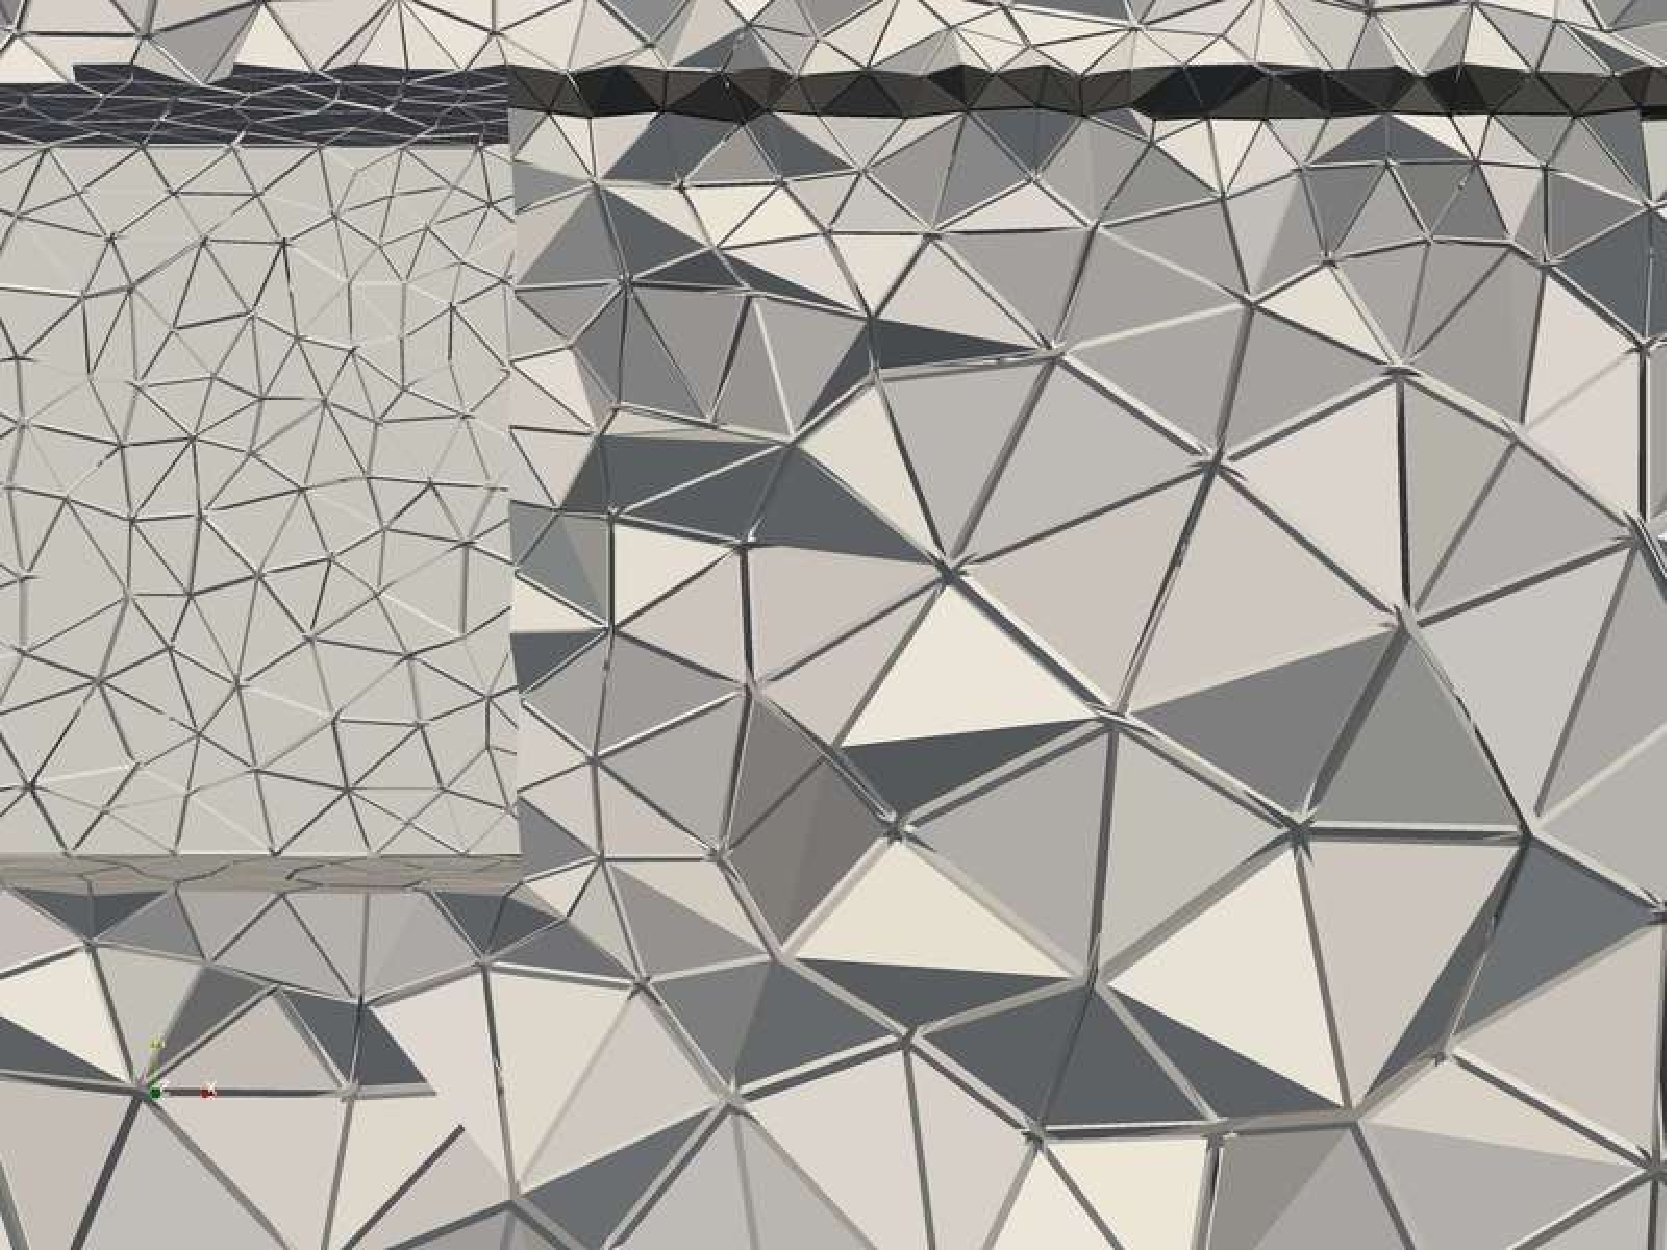
\includegraphics[height=0.24\linewidth]{chapters/hoffman-2/pdf/force_smooth01.pdf} &
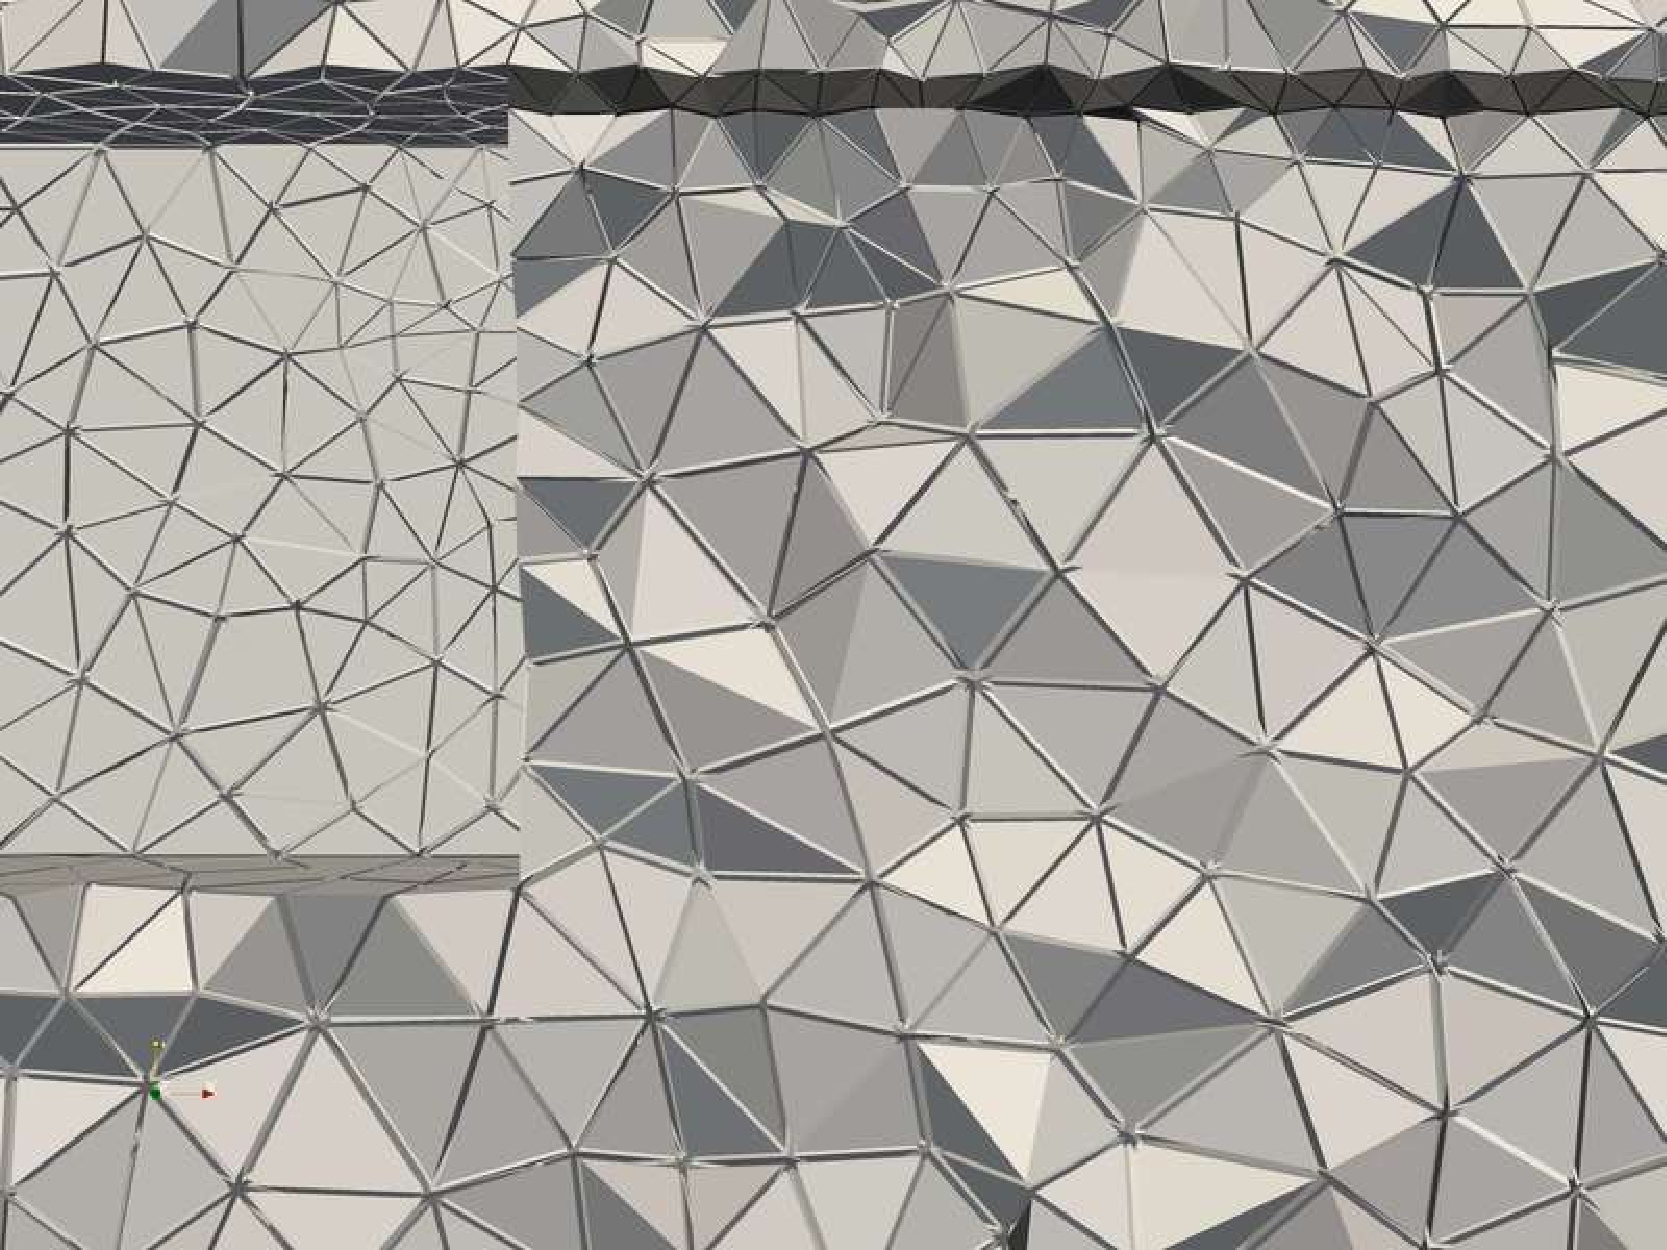
\includegraphics[height=0.24\linewidth]{chapters/hoffman-2/pdf/force_hybrid01.pdf}\\
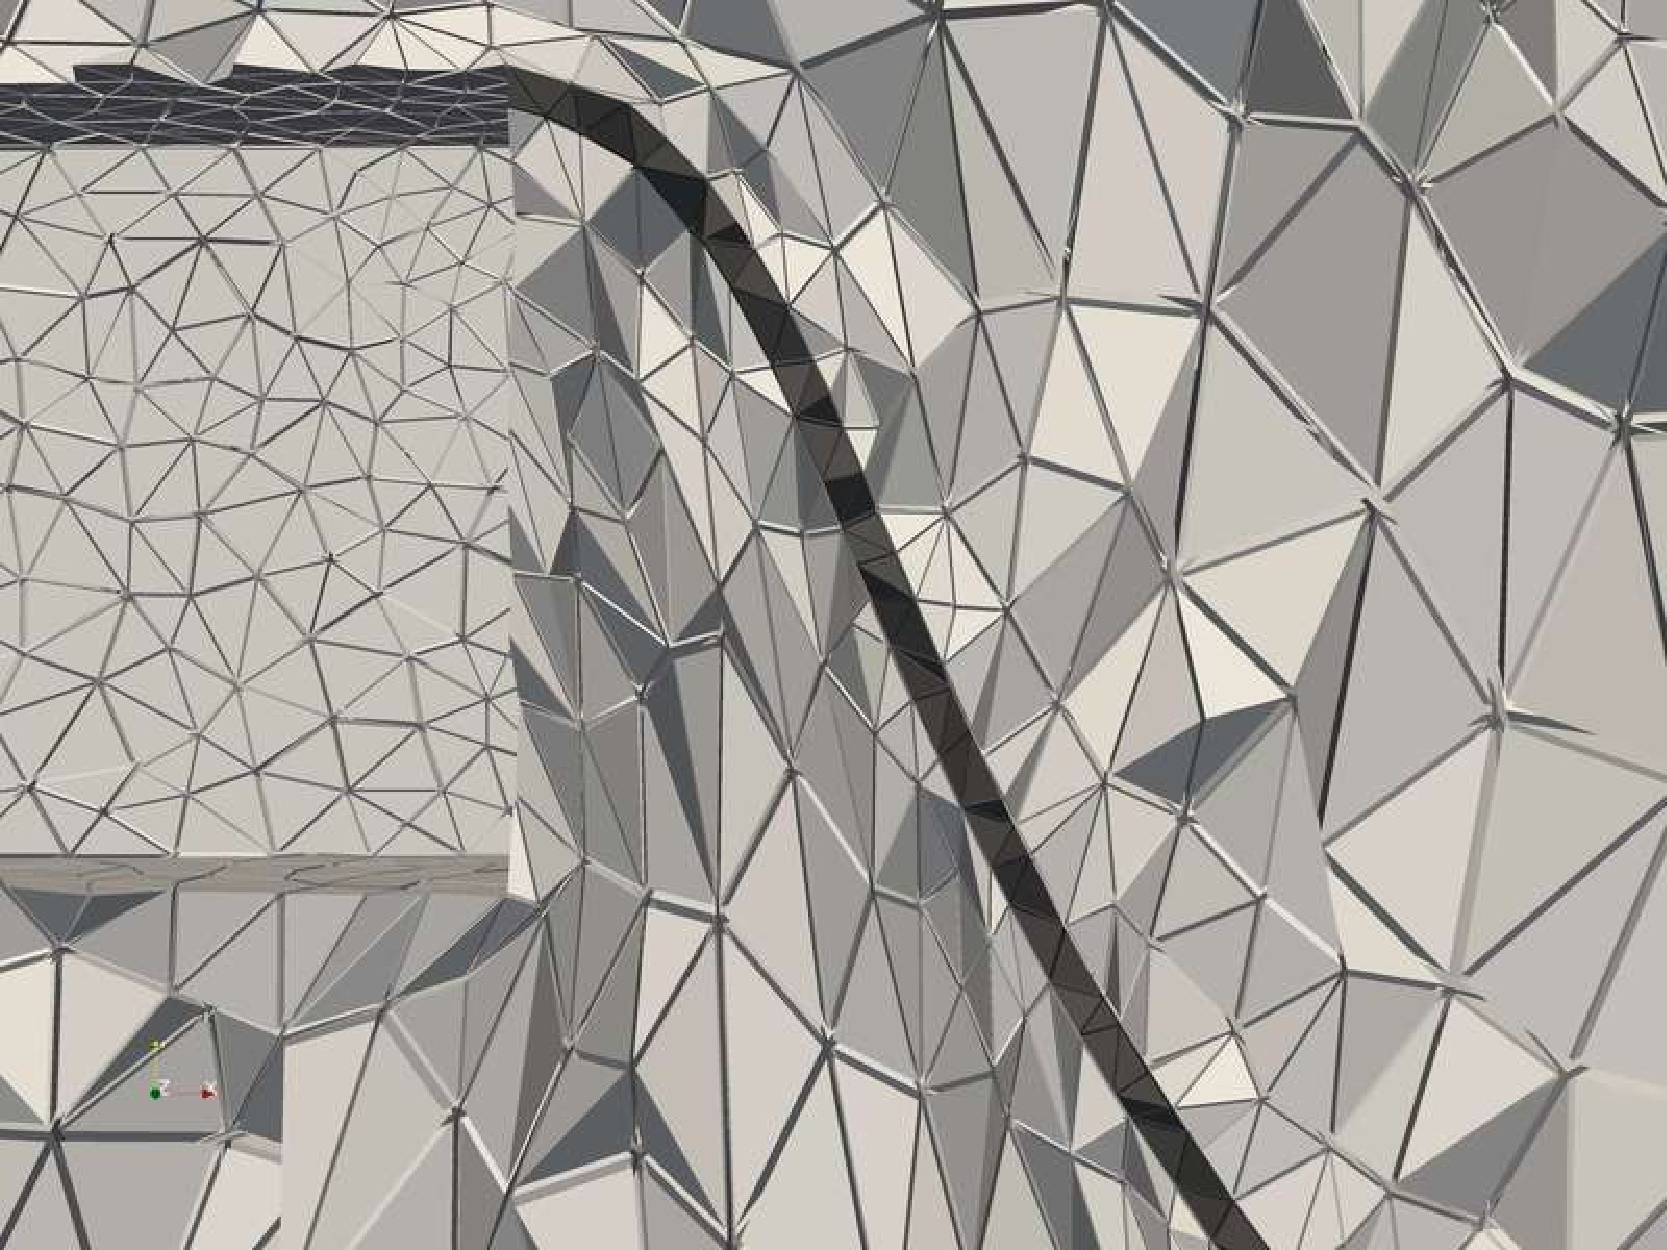
\includegraphics[height=0.24\linewidth]{chapters/hoffman-2/pdf/force_smooth02.pdf} &
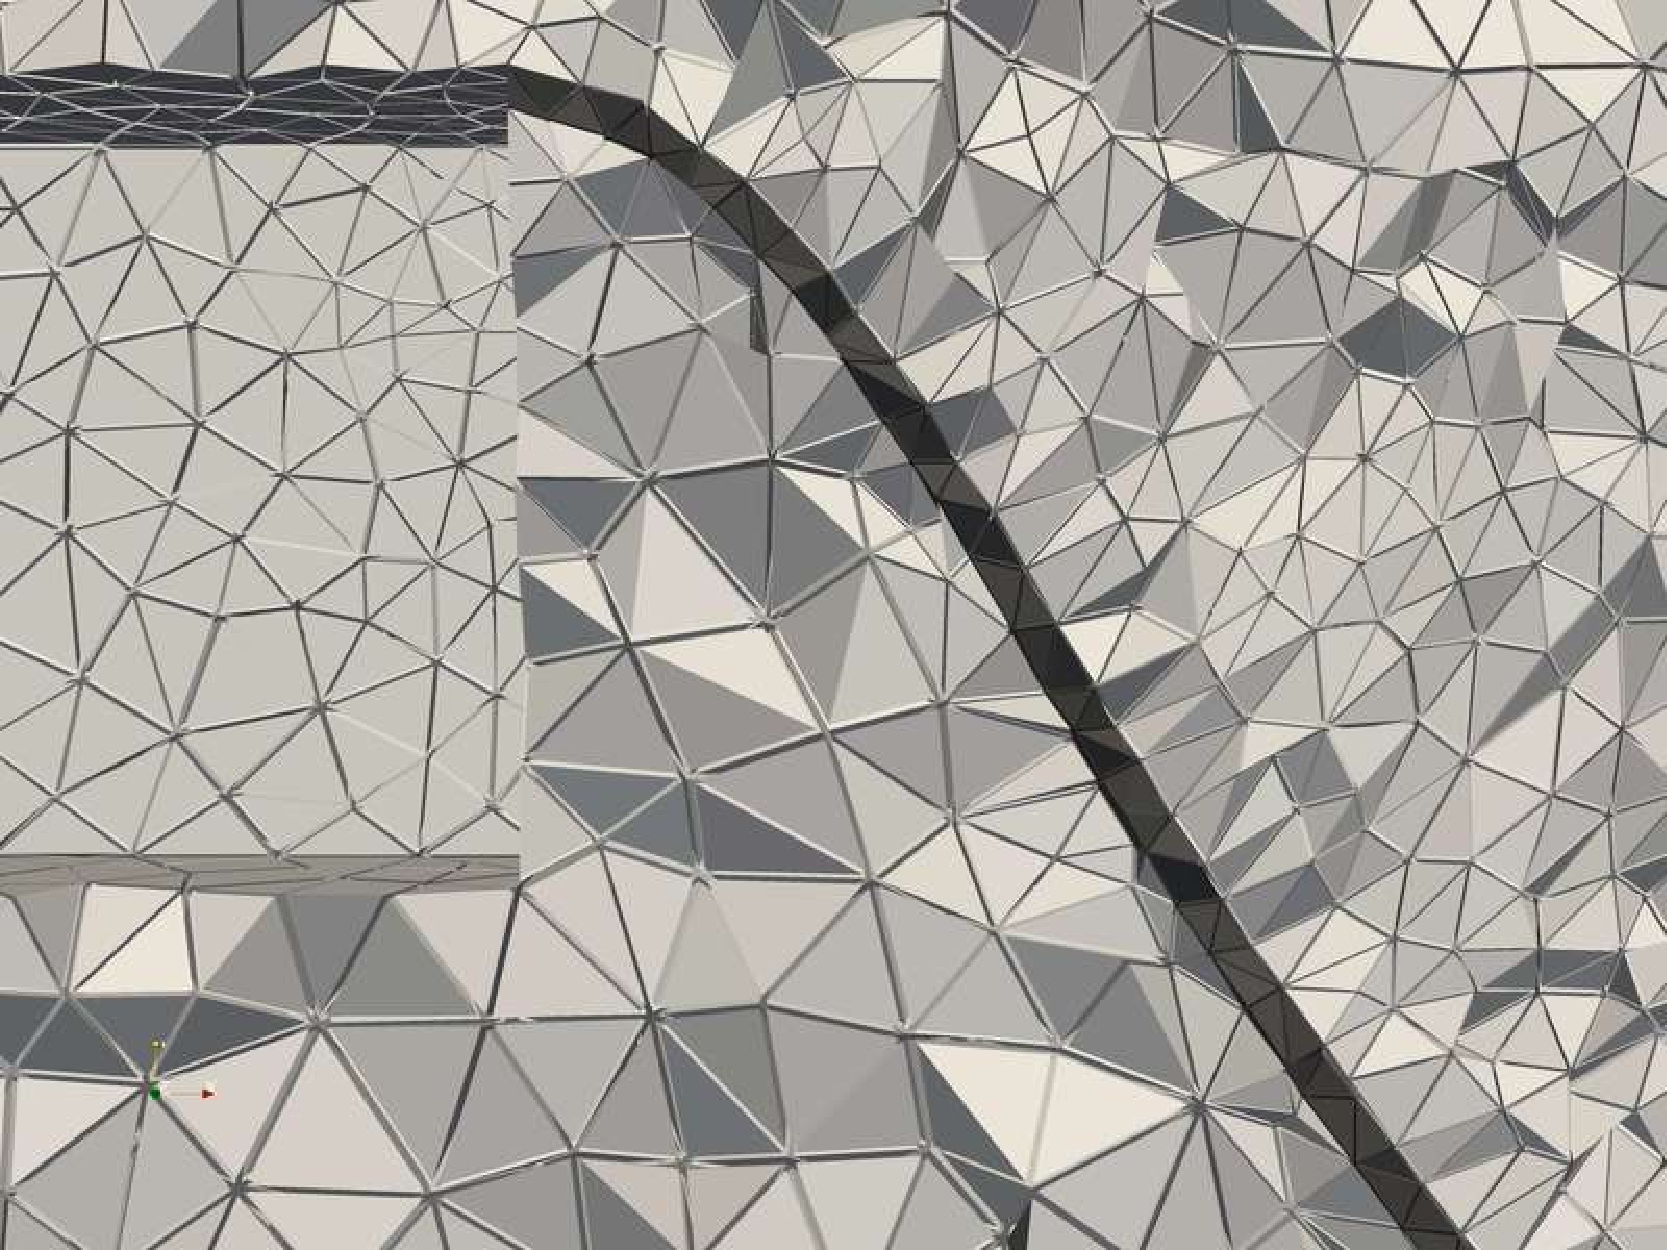
\includegraphics[height=0.24\linewidth]{chapters/hoffman-2/pdf/force_hybrid02.pdf}\\
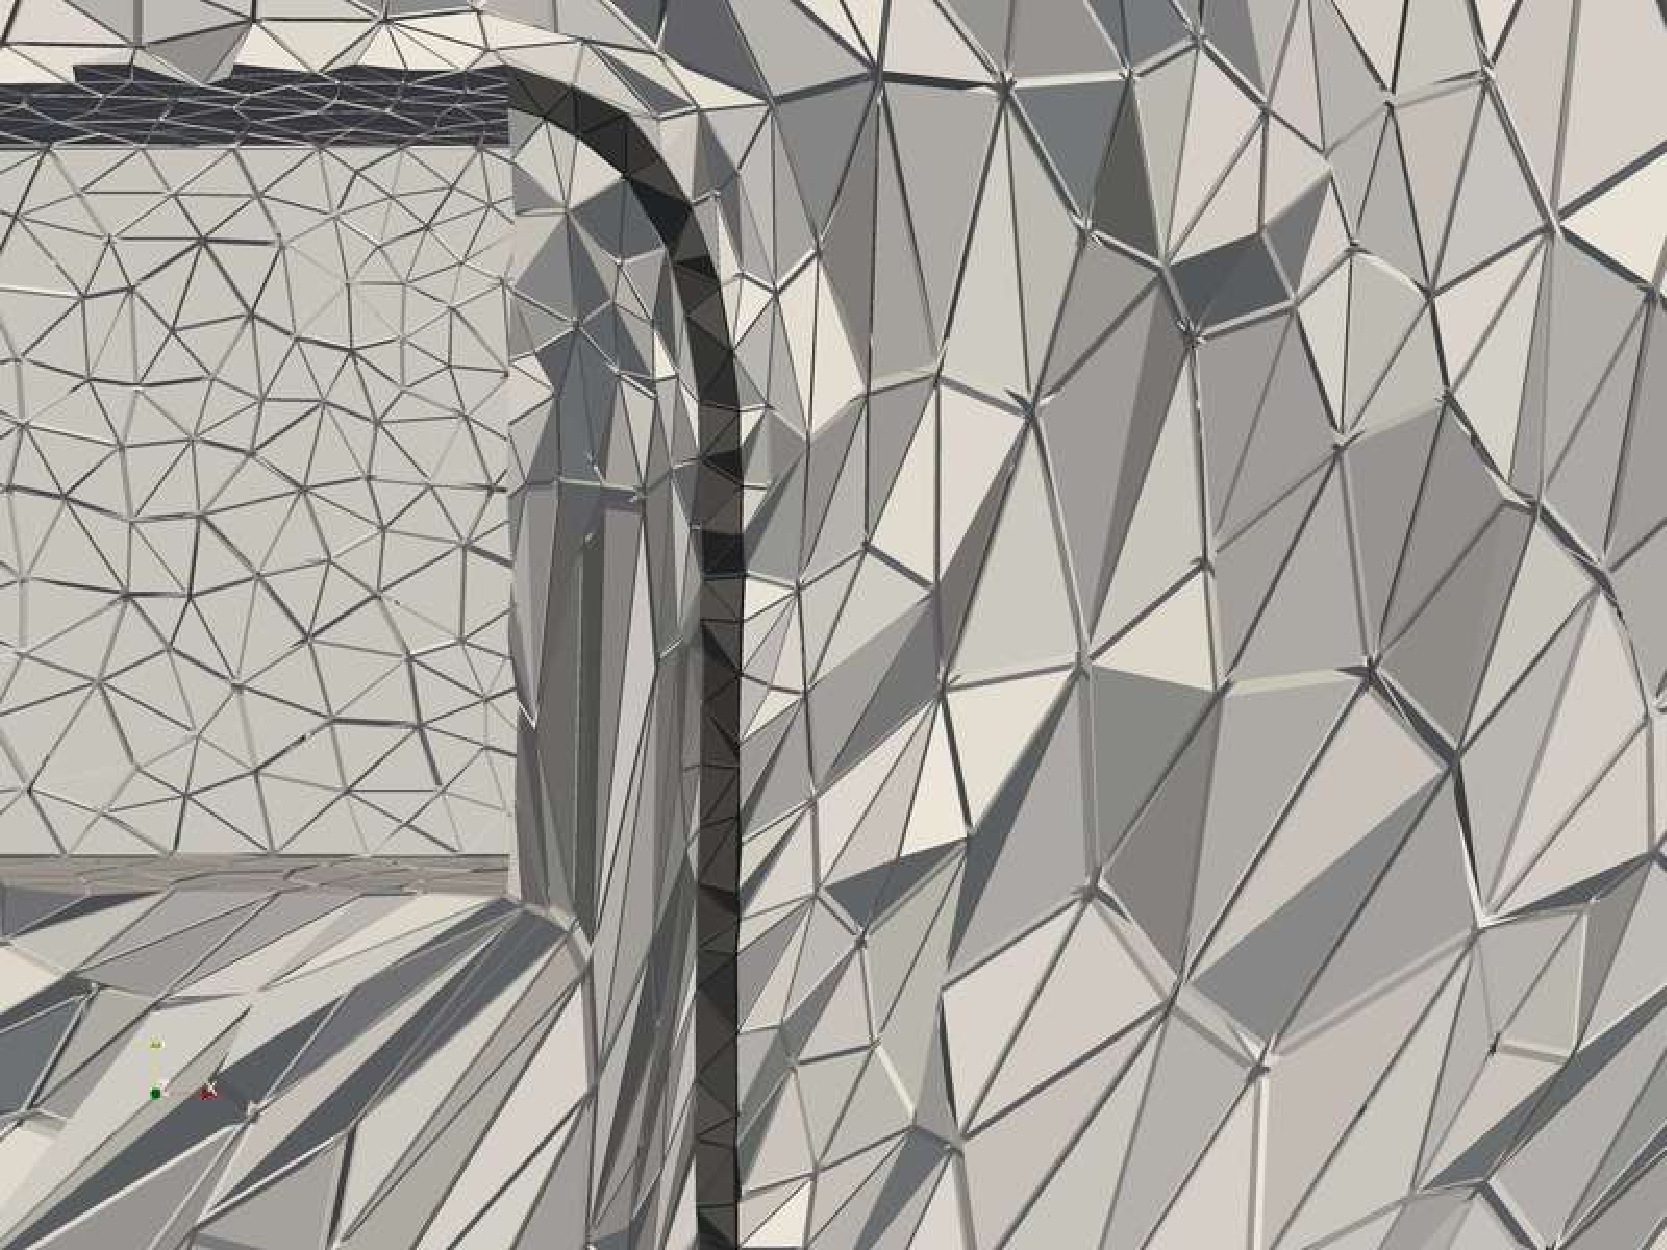
\includegraphics[height=0.24\linewidth]{chapters/hoffman-2/pdf/force_smooth03.pdf} &
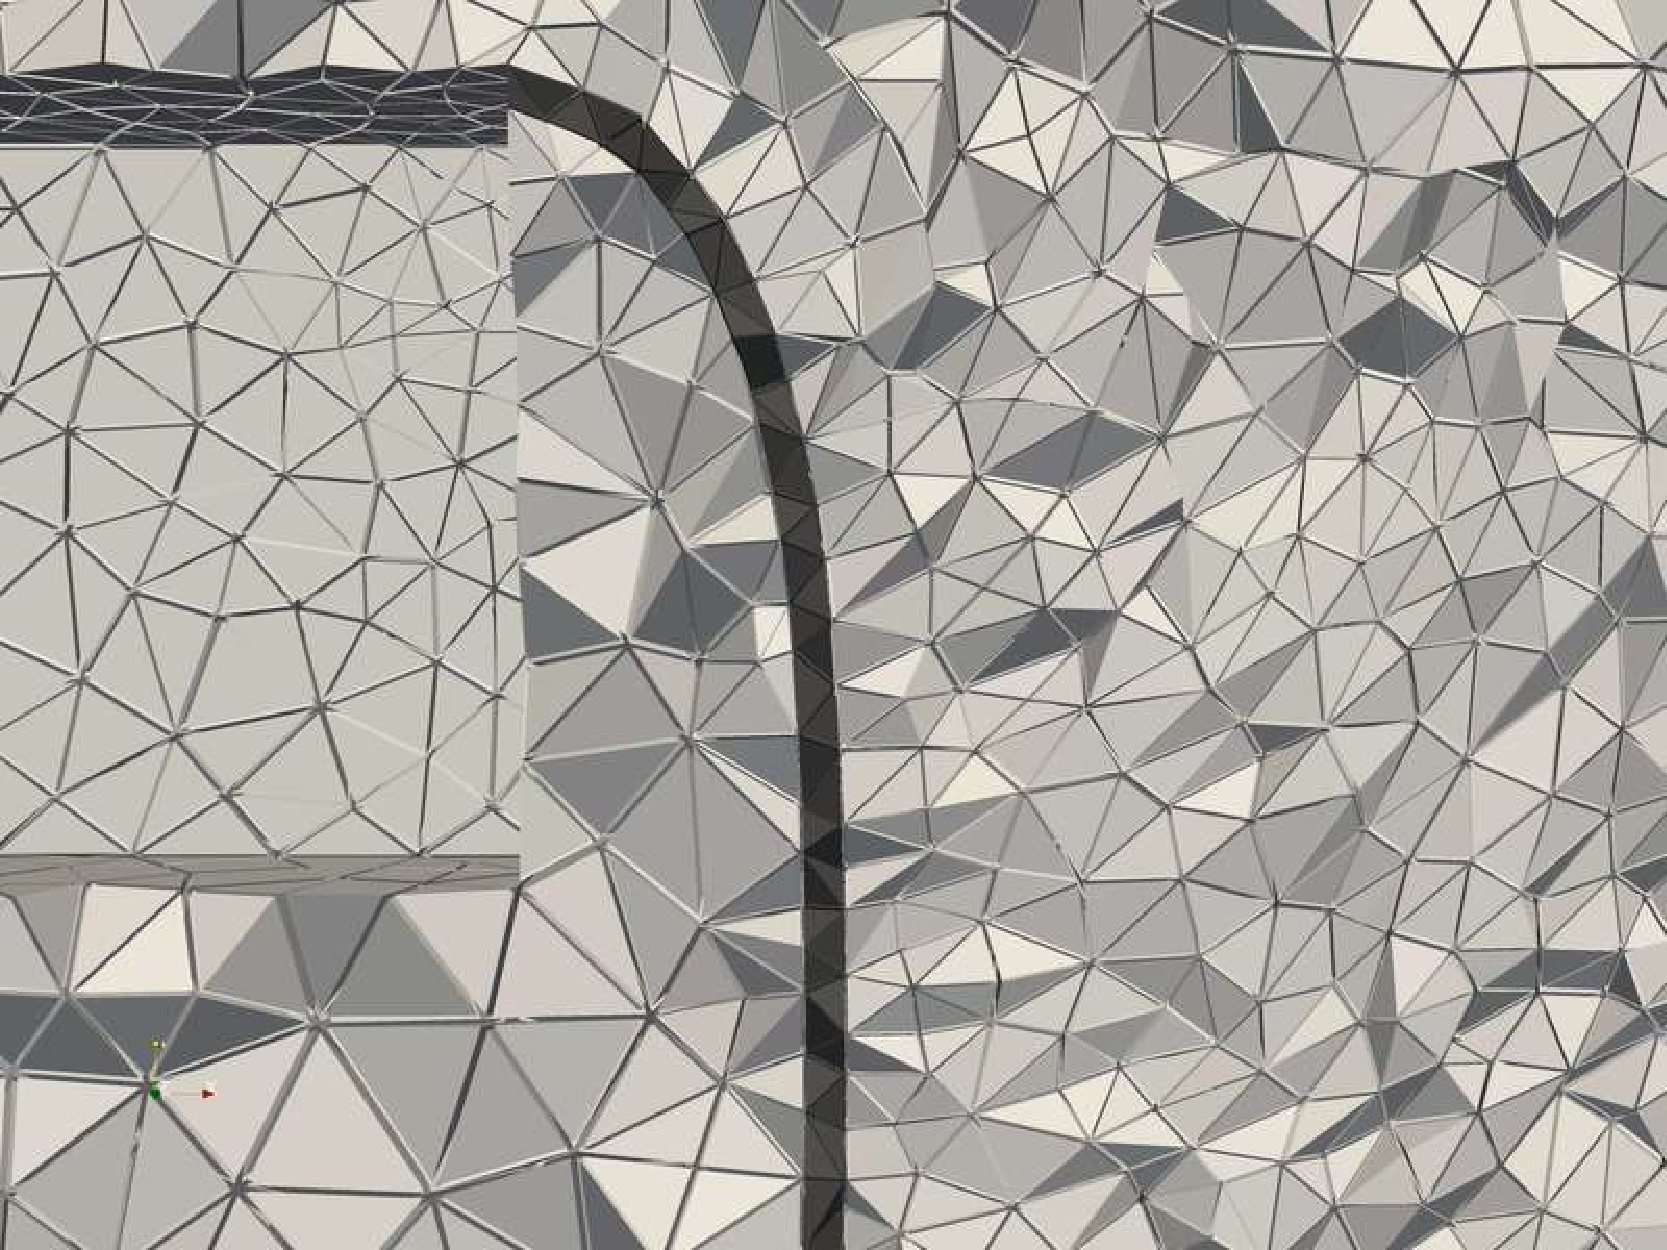
\includegraphics[height=0.24\linewidth]{chapters/hoffman-2/pdf/force_hybrid03.pdf}\\
(a) & (b)
\end{tabular}
\end{center}
\caption{Robustness test with (a) elastic smoothing and (b) mesh adaptation. Note the badly shaped cells squeezed between the cube and flag.}
\label{fig:flag_robustness}
\end{figure}

\begin{figure}[!h]
\begin{lstlisting}
  /// Optimize cell quality according to elastic variant of UC model
  class ElasticSmoother
  {
  public:

    ElasticSmoother(Mesh& mesh);

    /// Smooth smoothed_cells giving mesh velocity W over time step k
    /// with h0 the prescribed cell size
    void smooth(MeshFunction<bool>& smoothed_cells,
		MeshFunction<bool>& masked_cells,
		MeshFunction<real>& h0,
		Function& W, real k);

    /// Extract submesh (for smoothing only marked cells)
    static void submesh(Mesh& mesh, Mesh& sub,
			MeshFunction<bool>& smoothed_cells,
			MeshFunction<int>& old2new_vertex,
			MeshFunction<int>& old2new_cell);

  }
\end{lstlisting}
\caption{
C++ class interface for {\tt ElasticSmoother}.
}
\label{code:ElasticSmoother}
\end{figure}

To maintain a discontinuous phase interface in the UC with
fluid-structure data, we define the mesh velocity $\beta_h$ as the
discrete velocity $U$ in the solid phase (specifically on the
interface). The mesh velocity in the fluid can be chosen more
arbitrarily, but has to satisfy mesh quality and size criteria. We
construct a cell quality optimization/smoothing method based on a pure
elastic variant of the UC.

We define the following requirements for the mesh velocity $\beta_h$:

\begin{enumerate}
\item
$\beta_h = U$ in the solid phase part of the mesh.
\item
Bounded mesh quality $Q$ in the fluid part of the mesh. Preferably the
mesh smoothing should improve $Q$ if possible.
\item
Maintain mesh size $h(x)$ close to $\hat{h}(x)$ given by a posteriori
error estimation in an adaptive algorithm.
%\item
%$\nabla \beta_h$ and $D_t \beta_h$ must be bounded.
\end{enumerate}

We formulate a simplistic variant of the UC model where we only
consider a solid, and we omit the incompressibility equation (see
listing \ref{code:FFC_ElasticSmoother}). We use a constitutive law
$\sigma = \mu(I - (FF^\top)^{-1})$ where we recall $F$ as the
deformation gradient. We use the update law: $D_t F^{-1} =
-F^{-1} \nabla u$ where we thus need an initial condition for $F$. We
set the initial condition $F_0 = \bar{F}$ where $\bar{F}$ is the
deformation gradient with regard to a scaled equilateral reference
cell, representing the optimal shape with quality $Q = 1$.

Solving the elastic model can thus be seen as optimizing for the
highest global quality $Q$ in the mesh. We also introduce a weight on
the Young's modulus $\mu$ for cells with low quality, penalizing high
average, but low local quality over mediocre global quality. We refer
to the source code for more details.

As an alternative to mesh smoothing we can consider using local mesh
modification operations (refinement, coarsening, swapping) on the mesh
to maintain the quality \cite{Comp`ereRemacleJanssonEtAl2009}
through {\tt MeshAdaptInterface}.

Unicorn provides the {\tt ElasticSmoother} class (see
listing \ref{code:ElasticSmoother}, which can be used to
smooth/optimize for quality all or part of the mesh.

We perform a robustness test of the elastic smoothing and the mesh
adaptivity shown in \ref{fig:flag_robustness} where we use the same
geometry as the turbulent 3D flag problem, but define 0 inflow
velocity and instead add a gravity body force to the flag to create a
very large deformation with the flag pointing straight down. Both the
elastic smoothing and the mesh adaptvity compute solutions, but as
expected, the elastic mesh smoothing eventually cannot control the
cell quality (there does not exist a mesh motion which can handle
large rigid body rotations while bounding the cell quality).

\subsection{\tt MeshAdaptInterface}

A critical component in the adaptive algorithm as described above is
{\em Mesh adaptivity}, which we define as constructing a mesh
satisfying a given mesh size function $h(x)$.

We start by presenting the Rivara recursive bisection
algorithm \cite{Rivara1992} as a basic choice for mesh adaptivity
(currently the only available choice for parallel mesh adaptivity),
but which can only refine and not coarsen. Then the more general
MAdLib is presented, which enables the full mesh adaptation to the
prescribed $h(x)$ through local mesh operations: edge split, edge
collapse and edge swap.

\paragraph{Rivara recursive bisection}

The Rivara algorithm bisects (splits) the longest edge of a cell, thus
replacing the cell with two new cells, and uses recursive bisection to
eliminate non-conforming cells with hanging nodes. A non-conforming
cell $K_1$ has a neighbor (incident) cell $K_2$ that has a vertex on
an edge of cell $K_1$.

\begin{algorithm}
\caption{The Rivara recursive bisection algorithm}
\label{alg:rivara}
\begin{algorithmic}
\Procedure{bisect}{$K$}
\State Split longest edge $e$
\While{$K_i(e)$ is non-conforming}
\State BISECT($K_i$)
\EndWhile
\EndProcedure
\end{algorithmic}
\end{algorithm}

The same algorithm holds in both 2D/3D (triangles/tetrahedra). In 2D,
it can be shown \cite{Rivara1992} that the algorithm terminates in a
finite number of steps, and that the minimum angle of the refined mesh
is at least half the minimum angle of the starting mesh. In practice
the algorithm produces excellent quality refined meshes both in 2D and
3D.

\paragraph{Local mesh operations: Madlib}

 \begin{figure}[!h]
 \begin{center}
 \begin{tabular}{cc}
 \centering
 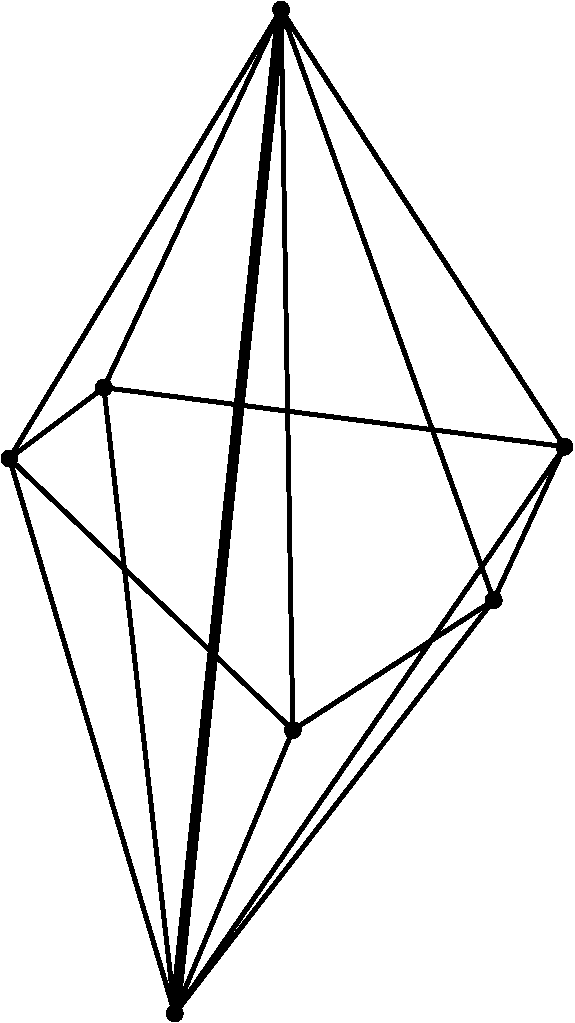
\includegraphics[height=3cm,width=6cm]{chapters/hoffman-2/pdf/swap.pdf} &
 \hspace{0.3cm}
 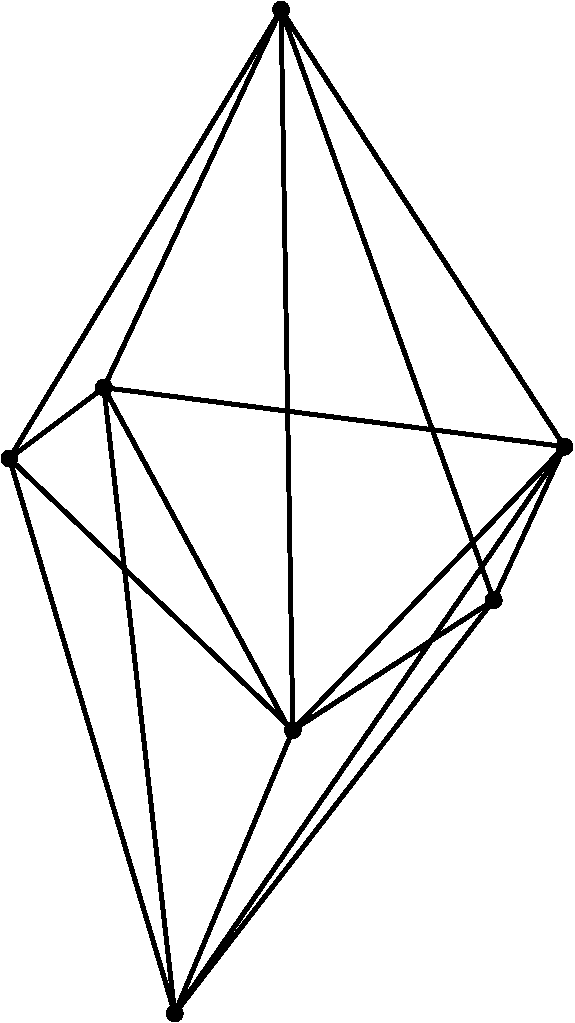
\includegraphics[height=3cm,width=6cm]{chapters/hoffman-2/pdf/swap_config1.pdf}
 \end{tabular}
 \end{center}
 \caption{Edge swap operation: (a) initial cavity with swap edge highlighted (b) possible configuration after the swap.}
 \label{fig:op:eswap}
 \end{figure}

Madlib incorporates an algorithm and implementation of {\bf mesh
adaptation} where a small set of local mesh modification operators are
defined such as edge split, edge collapse and edge swap. A mesh
adaptation algorithm is defined which uses this set of local operators
in a control loop to satisfy a prescribed size field $h(x)$ and
quality tolerance. Edge swapping is the key operator for improving
quality of cells, for example around a vertex with a large number of
connected edges.

In the formulation of finite element methods it is typically assumed
that the cell size of a computational mesh can be freely modified to
satisfy a desired size field $h(x)$ or to allow mesh motion. In
state-of-the-art finite element software implementations this is
seldom the case, where typically only limited operations are allowed
\cite{BangerthHartmannKanschat2007, COMSOL2009}, (local mesh refinement),
or a separate often complex, closed and ad-hoc mesh generation
implementation is used to re-generate meshes.

The mesh adaptation algorithm in Madlib gives the freedom to adapt to
a specified size field using local mesh operations. The implementation
is published as free software/open source allowing other research to
build on the results and scientific repeatability of numerical
experiments.

Unicorn provides the {\tt MeshAdaptInterface} class (see
listing \ref{code:MeshAdaptInterface}, where one can subclass and
implement virtual functions to control the mesh adaptation.

We perform a robustness test of the elastic smoothing and the mesh
adaptivity shown in \ref{fig:flag_robustness}, see a more detailed
description in the elastic smoothing section.


\begin{figure}[!h]
\begin{lstlisting}
  /// Interface to MAdLib for mesh adaptation using local operations
  /// Subclass and implement the virtual functions
  class MeshAdaptInterface
  {
  public:
    MeshAdaptInterface(Mesh *);

  protected:
    /// Start mesh adaptation algorithm
    void adaptMesh();

    /// Give cell size field
    virtual void updateSizeField() = 0;

    /// Allocate and deallocate solver data
    virtual void deallocateData() = 0;
    virtual void allocateAndComputeData() = 0;

    /// Constrain entities not to be adapted
    void constrainExternalBoundaries();
    void constrainInternalBoundaries();

    /// Add functions to be automatically interpolated
    void addFunction(string name, Function** f);
    void clearFunctions();
  };
}
\end{lstlisting}
\caption{
C++ class interface for {\tt MeshAdaptInterface}.
}
\label{code:MeshAdaptInterface}
\end{figure}



\section{Solving continuum mechanics problems}

In this section we give use cases for modeling and solving continuum
mechanics problems using the Unicorn technology. We start with a use
case for solving a fluid-structure problem without adaptivity, where
we cover modeling of geometry and subdomains, coefficients, dynamic
allocation of PDE data for mesh adaptivity and specification of main
program (interface to running the solver). Next, we present a use case
for solving a turbulent pure fluid problem with adaptivity, where we
cover modeling of data for the dual problem, the adaptive loop, and
specifying slip/friction boundary conditions for modeling turbulent
boundary layers.

\lstset{language=C++,frame=ltrb,framesep=5pt,basicstyle=\footnotesize,
 keywordstyle=\ttfamily\color{OliveGreen},
 identifierstyle=\ttfamily\color{CadetBlue}\bfseries,
 commentstyle=\color{Brown},
 stringstyle=\ttfamily,
 showstringspaces=ture}

\subsection{Fluid-structure}

\begin{figure}[!ht]
\begin{center}
\begin{tabular}{cc}
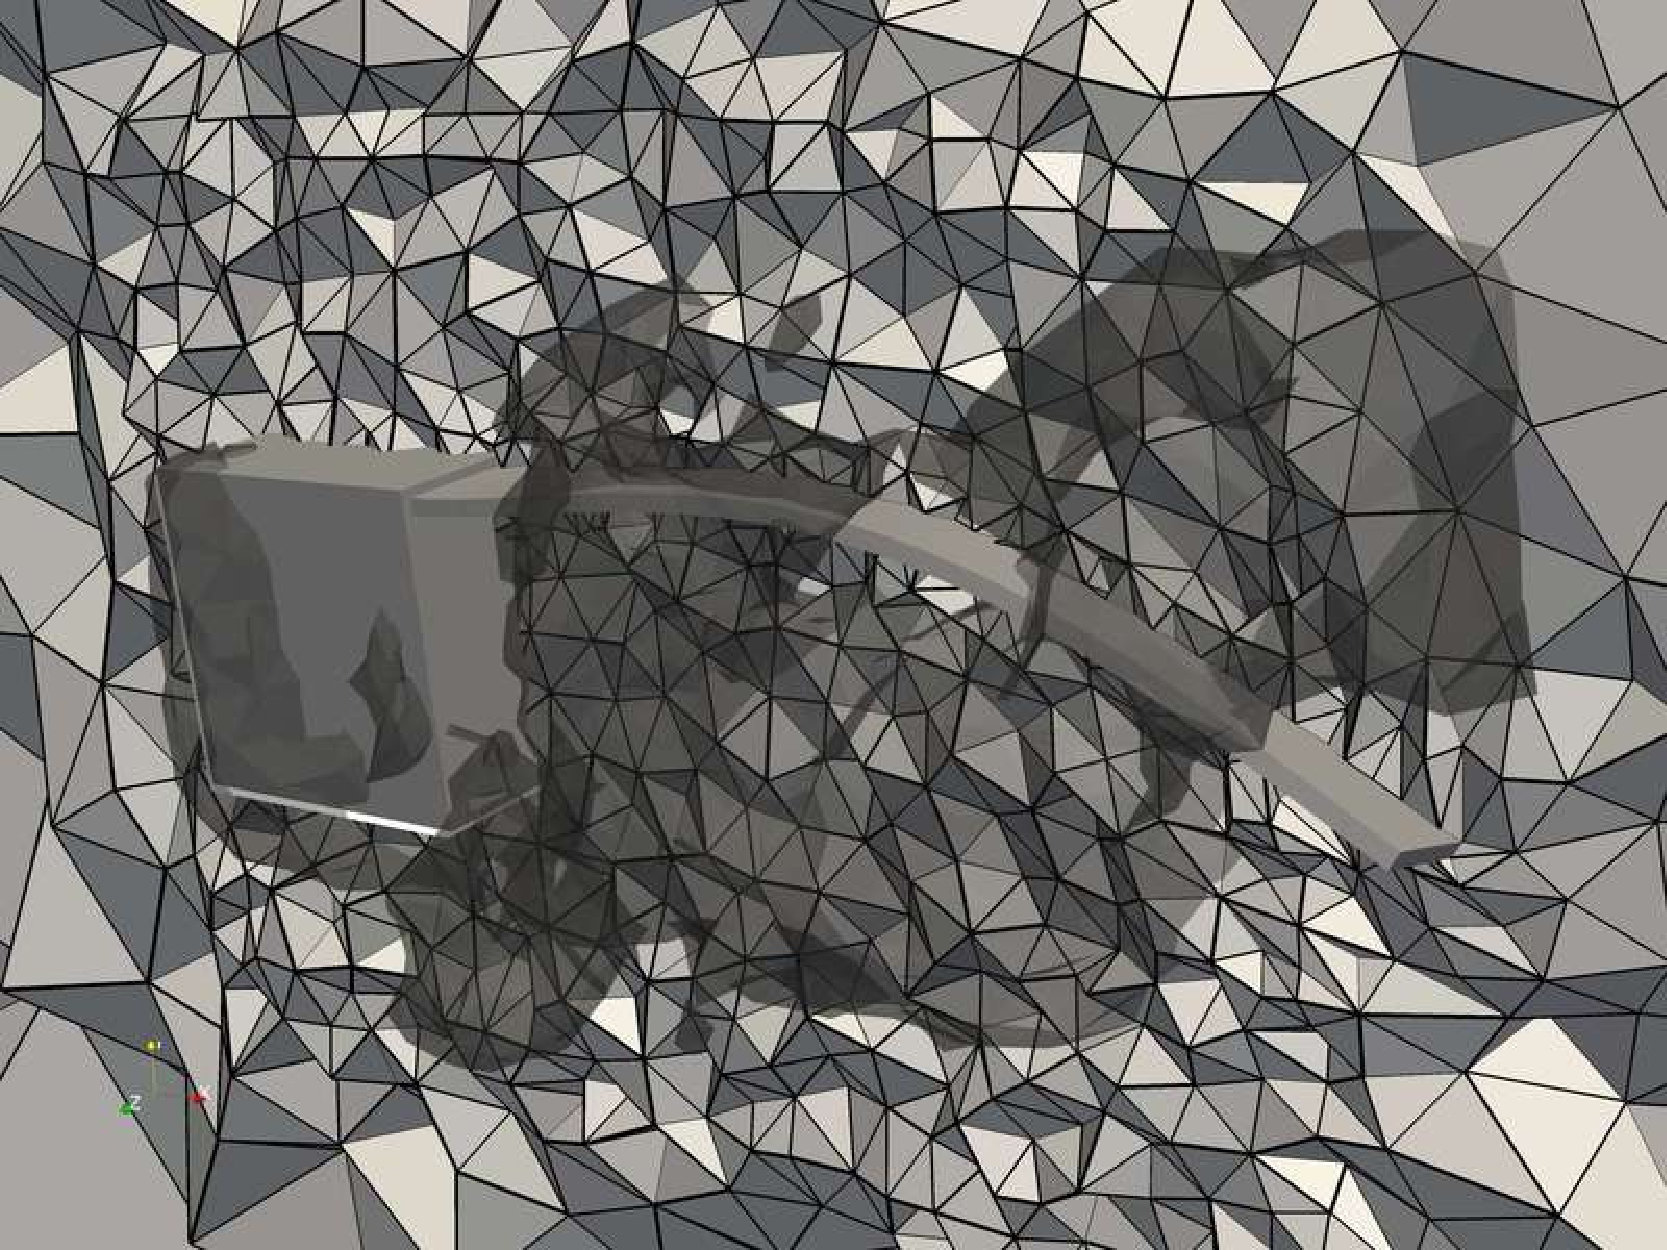
\includegraphics[width=0.5\linewidth]{chapters/hoffman-2/pdf/flag_smooth05.pdf} &
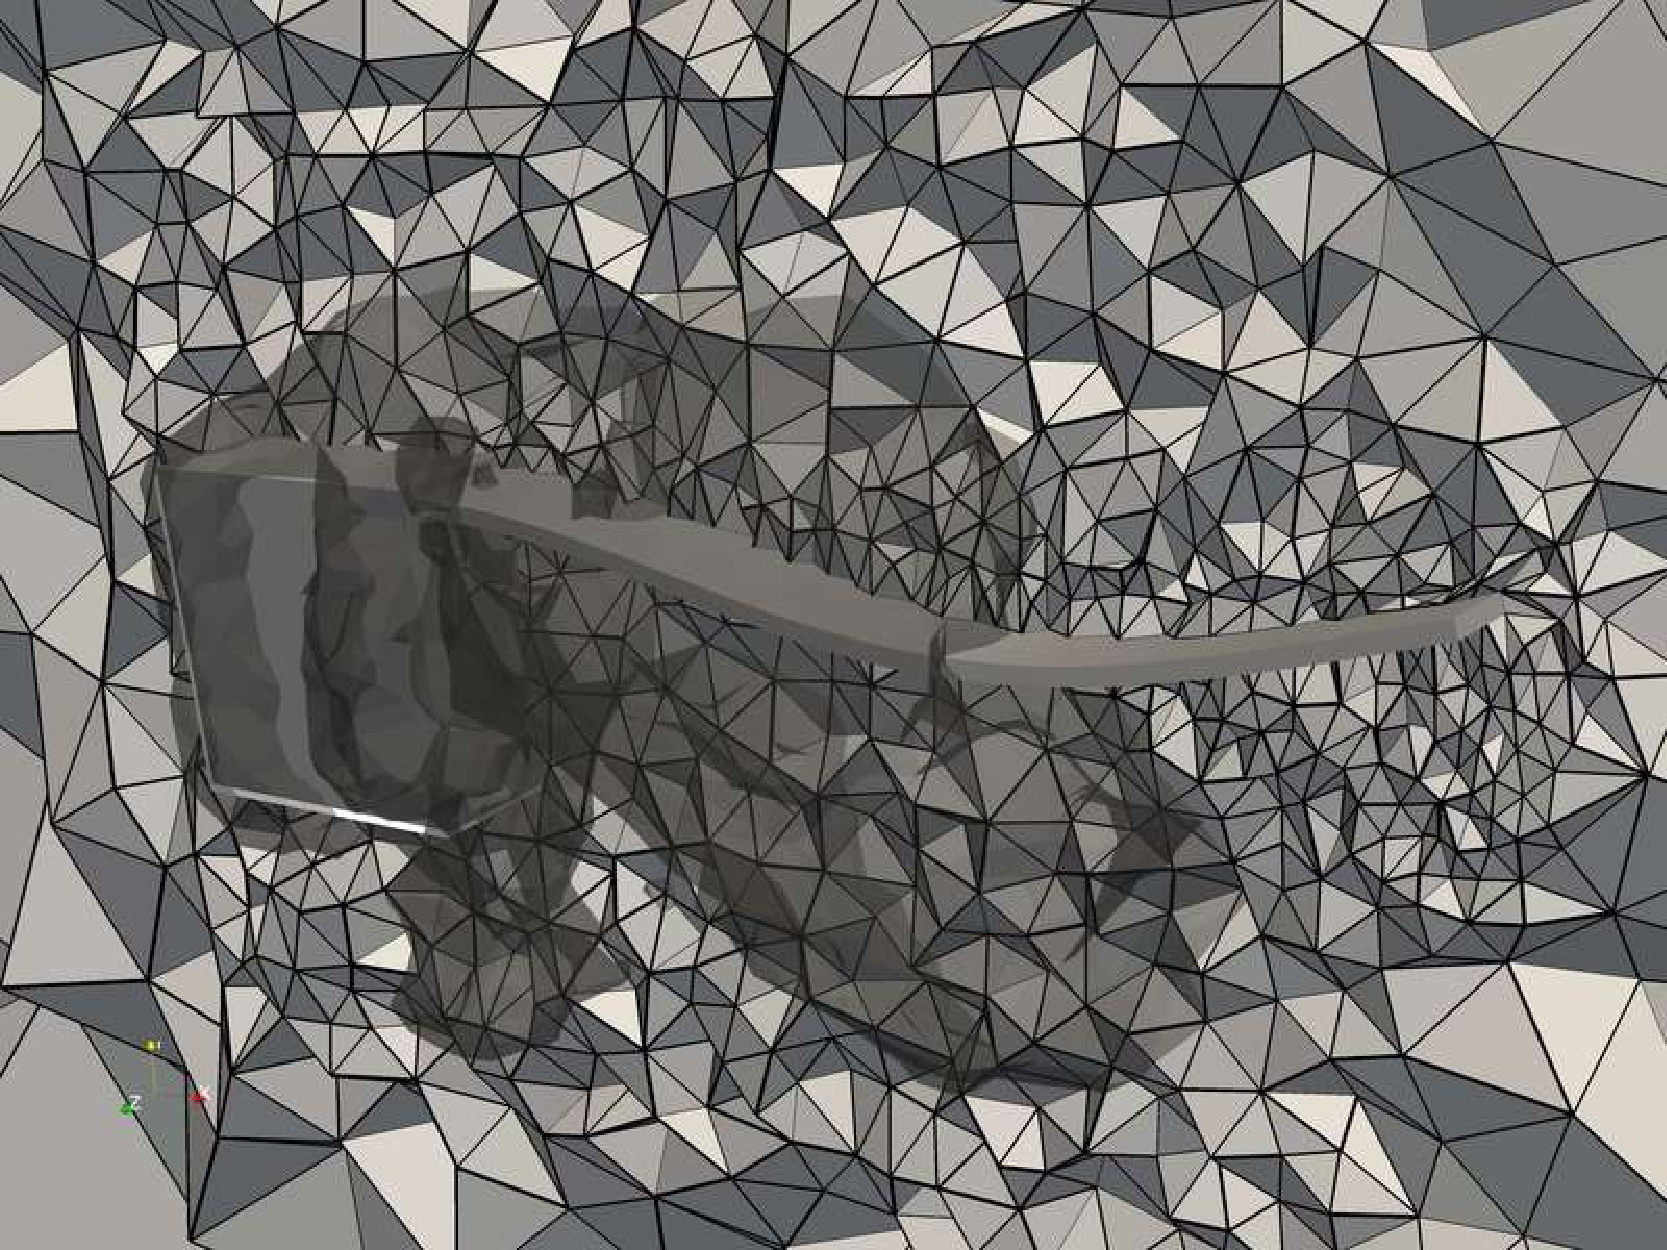
\includegraphics[width=0.5\linewidth]{chapters/hoffman-2/pdf/flag_hybrid05.pdf}\\
(a) & (b)
\end{tabular}
\end{center}
\caption{Snapshot of flag simulation FSI use case with (a) elastic smoothing and
  (b) dynamic mesh adaptation. A cut of the mesh is shown together with an
  isosurface of the pressure to visualize the flow.}
\label{fig:flag_snapshot}
\end{figure}

We here give a use case of solving a fluid-structure continuum
mechanics problem, where the user specifies data for modeling the
problem, and illustrates interfaces and expected outcomes. We divide
the use case into 4 parts:

\begin{description}
\item[Geometry and subdomains]
\ \\
The user specifies possible geometrical parameters and defines
subdomains. We note that for complex geometries the user may omit
geometry information and specify subdomain markers as data files.
\item[Coefficients]
\ \\
Known coefficients such as a force function and boundary conditions
are declared.
\item[PDE data]
\ \\
The user subclasses a PDEData class and specifies how the PDE data is
constructed and destroyed. This construction/destruction may happen
during the simulation if the mesh is adapted.
\item[main program]
\ \\
The user implements the main program and declares and passes data to
to the solver.
\end{description}

\subsection{Adaptivity}

We continue with a use case for adaptive solution of a pure fluid
turbulent flow problem: flow around a 3D cylinder. The implementation
of the problem is very similar to the fluid-structure case (just with
pure fluid data), but with 3 important additions:
\begin{description}
\item[Dual problem]
\ \\
To compute the error estimate required by the adaptive algorithm, we
must solve a dual problem generated by the primal problem and an
output quantity $\psi$. Since the dual problem is similar in form to
the primal problem, we implement both as variants of the same solver.

In this case we are interested in computing drag, which gives $\psi$
as a boundary condition for the dual problem:

\begin{lstlisting}
CylinderBoundary cb;
SubSystem xcomp(0);
Function minus_one(mesh, -1.0);

DirichletBC dual_bc0(minus_one, mesh, cb, xcomp);

Array <BoundaryCondition*> dual_bc_mom;
dual_bc_mom.push_back(&dual_bc0);
\end{lstlisting}


\item[Adaptive loop]
\ \\
We construct the program to compute one iteration of the adaptive
loop: solve primal problem, solve dual problem, compute error estimate
and check if tolerance is satisfied, compute adapted mesh. We can then
run the adaptive loop simply by a loop which runs the program (here in
Python which we also use to move data according to iteration number):

\lstset{language=Python,frame=ltrb,framesep=5pt,basicstyle=\footnotesize,
 keywordstyle=\ttfamily\color{OliveGreen},
 identifierstyle=\ttfamily\color{CadetBlue}\bfseries,
 commentstyle=\color{Brown},
 stringstyle=\ttfamily,
 showstringspaces=ture}

\begin{lstlisting}
offset = 0
N = 20

for i in range(offset, N):
    dirname = ``iter_%2.2d'' % i
    mkdir(dirname)

    system(``./unicorn-cylinder > log'')
    for file in glob(``./*.vtu''):
    move(file, dirname)
    for file in glob(``./*.pvd''):
    move(file, dirname)
\end{lstlisting}

\lstset{language=C++,frame=ltrb,framesep=5pt,basicstyle=\footnotesize,
 keywordstyle=\ttfamily\color{OliveGreen},
 identifierstyle=\ttfamily\color{CadetBlue}\bfseries,
 commentstyle=\color{Brown},
 stringstyle=\ttfamily,
 showstringspaces=ture}

\item[Slip boundary condition]
\ \\
For turbulent flow we model the boundary layer as a friction boundary
condition. We specify the normal component as a string slip boundary
condition used just as a regular Dirichlet boundary condition. The
{\tt xcomp} variable denotes an offset for the first velocity
component in a system (for compressible Euler the system is [density,
velocity, energy], and we would thus give component 2 as offset).

\begin{lstlisting}
SlipBoundary sb;
SubSystem xcomp(0);

SlipBC slip_bc(mesh, sb, xcomp);

Array <BoundaryCondition*> primal_bc_mom;
primal_bc_mom.push_back(&slip_bc);
\end{lstlisting}


\end{description}


\begin{figure}[!h]
\begin{lstlisting}
#include <dolfin.h>
#include <unicorn/FSIPDE.h>

using namespace dolfin;
using namespace dolfin::unicorn;

real bmarg = 1.0e-3 + DOLFIN_EPS;

namespace Geo
{
  // Geometry details /////////////////////////////////////////////////
  real box_L = 3.0;
  real box_H = 2.0;
  real box_W = 2.0;

  real xmin = 0.0; real xmax = box_L;
  real ymin = 0.0; real ymax = box_H;
  real zmin = 0.0; real zmax = box_W;
}

// Sub domain for inflow
class InflowBoundary3D : public SubDomain
{
public:
  bool inside(const real* p, bool on_boundary) const
  {
    return on_boundary && (p[0] < Geo::xmax - bmarg);
  }
};

// Sub domain for outflow
class OutflowBoundary3D : public SubDomain
{
public:
  bool inside(const real* p, bool on_boundary) const
  {
    return on_boundary && (p[0] > Geo::xmax - bmarg);
  }
};
\end{lstlisting}
\caption{Part 1 of Unicorn solver FSI use case: geometry and subdomains.}
\end{figure}

\begin{figure}[!h]
\begin{lstlisting}
// Force term
class ForceFunction : public Function
{
public:
  ForceFunction(Mesh& mesh, TimeDependent& td) : Function(mesh), td(td) {}
  void eval(real* values, const real* x) const
  {
    int d = cell().dim();

    for(int i = 0; i < d; i++)
    {
      values[i] = 0.0;
    }
  }

  TimeDependent& td;
};

// Boundary condition for momentum equation
class BC_Momentum_3D : public Function
{
public:
  BC_Momentum_3D(Mesh& mesh, TimeDependent& td) :
    Function(mesh), td(td) {}
  void eval(real* values, const real* x) const
  {
    int d = cell().dim();

    for(int i = 0; i < d; i++)
    {
      values[i] = 0.0;
    }
    if (x[0] < (Geo::xmin + bmarg))
      values[0] = 100.0;
  }

  TimeDependent& td;
};


// Initial condition for phase variable
class BisectionFunction : public Function
{
public:
  BisectionFunction(Mesh& mesh) : Function(mesh) {}
  void eval(real* values, const real* p) const
  {
    // NB: We specify the phase variable as xml data so
    // this function is not used

    bool condition = true;

    if (condition)
      values[0] = 0.0;
    else
      values[0] = 1.0;
  }
};
\end{lstlisting}
\caption{Part 2 of Unicorn solver FSI use case: coefficients.}
\end{figure}

\begin{figure}[!h]
\begin{lstlisting}
class FlagData : public PDEData
{
public:
  void create(Mesh& mesh)
  {
    bcf_mom = new BC_Momentum_3D(mesh, td);
    bcf_con = new BC_Continuity_3D(mesh);
    f = new ForceFunction(mesh, td);

    bisect = new BisectionFunction(mesh);
    zero = new Function(mesh, 0.0);

    bc_mom0 = new DirichletBC(*bcf_mom, mesh,
			      iboundary);
    bc_con0 = new DirichletBC(*bcf_con, mesh,
			      oboundary);

    bc_mom.clear();
    bc_con.clear();

    bc_mom.push_back(bc_mom0);
    bc_con.push_back(bc_con0);
  }

  void destroy()
  {
    delete bcf_mom;
    delete bcf_con;
    delete f;
    delete bisect;
    delete zero;

    delete bc_mom0;
    delete bc_con0;
  }

  Function* bcf_mom;
  Function* bcf_con;
  Function* f;
  Function* bisect;
  Function* zero;

  DirichletBC* bc_mom0;
  DirichletBC* bc_con0;

  Array <BoundaryCondition*> bc_mom;
  Array <BoundaryCondition*> bc_con;

  InflowBoundary3D iboundary;
  OutflowBoundary3D oboundary;

  TimeDependent td;
};
\end{lstlisting}
\caption{Part 3 of Unicorn solver FSI use case: problem data.}
\end{figure}


\begin{figure}[!h]
\begin{lstlisting}
int main()
{
  Mesh mesh("flag.xml");

  real nu = 0.0;
  real nus = 0.5;
  real rhof = 1.0;
  real rhos = 1.0;

  real E = 1.0e6;

  real T = 0.2;

  dolfin::set("ODE number of samples", 500);

  Function U, U0;

  real u_bar = 100.0;

  FlagData pdedata;

  ICNSPDE pde(U, U0, &(pdedata.bisect), mesh,
	      pdedata.bc_mom, pdedata.bc_con,
	      &(pdedata.f), T, nu, E, nus, rhof, rhos,
	      u_bar, pdedata.td, &pdedata);

  // Compute solution
  pde.solve(U, U0);

  return 0;
}
\end{lstlisting}
\caption{Part 4 of FSI use case: main program, passing data to solver.}
\end{figure}


